\documentclass[11pt, oneside]{article}
\usepackage[utf8]{inputenc}                        % utf8
\usepackage[T1]{fontenc}                           % fix font encoding
\usepackage[english]{babel}                        % language
\usepackage{titling, geometry, hyperref, fancyhdr, algorithm, sidecap, multirow}
\usepackage{amsmath, amssymb, amsthm}              % ams mathematical packages
\usepackage{physics, mathtools, bm}                % extra math packages
\usepackage{graphicx, subcaption, wrapfig}         % images
\usepackage{fvextra, textcomp, CJKutf8}            % misc. text formatting
\usepackage[autostyle, english=american]{csquotes} % quotes
\usepackage[shortlabels]{enumitem}                 % lists
\usepackage{tikz, pgfplots, tikz-network}          % plots and graphs
\usepackage[noend]{algpseudocode}                  % algorithm psuedocode
\usepackage[cache=true]{minted}                    % source code
\usepackage[style=ieee]{biblatex}                  % bibliography
\geometry{a4paper}

\pgfplotsset{compat=1.17}                          % version of pgfplots

\hypersetup{
  colorlinks=true,
  urlcolor=cyan,
  linkcolor=magenta
}

\setminted[]{
  linenos=false,
  breaklines=true,
  encoding=utf8,
  fontsize=\normalsize,
  frame=lines,
  framesep=2mm
}

% https://tex.stackexchange.com/questions/343494/minted-red-box-around-greek-characters
\makeatletter
\AtBeginEnvironment{minted}{\dontdofcolorbox}
\def\dontdofcolorbox{\renewcommand\fcolorbox[4][]{##4}}
\makeatother

\graphicspath{{./images/}}
\addbibresource{ref.bib}

\newcommand{\emphasis}[1]{\textbf{\textit{#1}}}
\DeclareMathOperator{\E}{E}
\DeclareMathOperator{\Var}{Var}

\theoremstyle{plain}
\newtheorem{theorem}{Theorem}[section]
\newtheorem{corollary}{Corollary}[theorem]
\newtheorem{lemma}[theorem]{Lemma}

\theoremstyle{definition}
\newtheorem{definition}{Definition}[section]
\renewcommand\qedsymbol{$\square$} 

\def\algorithmautorefname{algorithm}

\title{Case Study of the Discord Mudae System}
\author{Stephen Huan}
\date{January 25, 2021}

\begin{document}
\maketitle
\setcounter{tocdepth}{3} % include subsubsection
{\hypersetup{linkcolor=black}
\tableofcontents
\listofalgorithms
}
% \listoffigures
\newpage

\section{Introduction} \label{sec:intro}
\href{https://discord.com/}{Discord} is a popular messaging platform
whose API is very useful, allowing many users to create \enquote{bots}.
These bots automate interactions with Discord users through text
and other means to perform a specific function. Among these bots is
\href{https://top.gg/bot/432610292342587392}{Mudae}, which allows the
user to play a simple game. One types in the \texttt{\$wa} command to
\enquote{roll}, which instructs Mudae to show a random character from
television shows. One can then \enquote{claim} a character, which means
they now have possession of the character. Note that one can roll 10
times per hour, but only claim once per 3 hours. Thus, there are 30
rolls per claim, and it is impossible to know \textit{a prori} when
to stop rolling and settle on a character.

Each character has a \emphasis{kakera value}, which is an objective
determination of value irrespective of the emotional value one might
attach to their favorite characters. Thus, our discussion centers around
maximizing kakera. Suppose one rolls a 100 kakera value character. Should
they stop rolling and claim this character, or continue rolling in hope of
getting a higher value later? To answer this central question, we must use
the methods of probability theory to analyze the kakera distribution.
\footnote{This problem is very similar to the secretary problem,
described in the appendix, \autoref{subsec:secretary}.}

\begin{SCfigure}[1][!h]
  \centering
  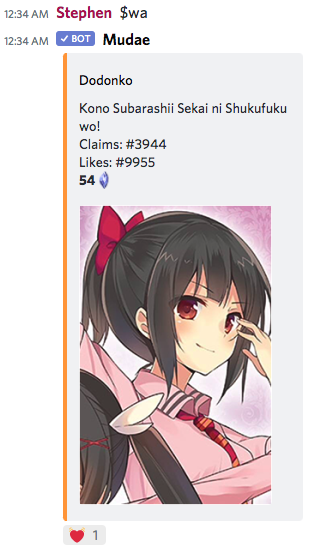
\includegraphics[scale=0.6]{mudae}
  \caption{An example roll. The character name (Dodonko) is at the top, and the
  show they are from under it (KonoSuba). The number left of the crystal icon
  indicates the kakera value, in this case 54. One clicks the heart icon under
  the Mudae modal to claim the character.}
\end{SCfigure}

\section{Probability Theory}
\textit{If you are already familiar with the basic concepts of probability
theory, e.g. random variables, PMFs, CMFs, expected value, and variance,
feel free to skip to the next \hyperref[subsec:computer]{section}.}

\subsection{Basic Definitions}
\begin{definition}
  A \textit{random variable} (r.v.) is formally a function assigning
  a value to an outcome, but can more intuitively be thought of as a
  \enquote{dispenser} of random values. We will denote random variables
  as a single uppercase letter, e.g. \( X \) or \( Z \).
  
  A random variable is \textit{continuous} if it dispenses infinite possible
  values (e.g. a random number between 0 and 1) and \textit{discrete} if it
  dispenses a finite number of possible values (e.g. a coin). We are dealing
  with a discrete space---the kakera values are integer and vary between 32
  and 1239, so we will focus on discrete random variables.
\end{definition}

\begin{definition}
  A \textit{probability mass function} (PMF) gives the probability that a
  random variable dispenses a value. We will denote a PMF associated with
  the random variable \( X \) as \( f_X(x) \), which gives the probability
  of the event \( x \) happening, \( p(X = x) \).
\end{definition}

\begin{definition}
  The \textit{cumulative mass function} (CMF) gives the probability that a
  random variable dispenses a value \textit{less than or equal} to a given
  value. We will denote a CMF associated with the random variable \( X \) as
  \( F_X(x) \), which gives \( p(X \leq x) \).
\end{definition}

\begin{definition}
  The \textit{expected value} is what we \enquote{expect} a random variable
  to dispense over many samples, or the average value. One way to compute
  this is: \[ \E[X] = \sum_{x \in X} x p(x) \] or each value times the
  probability it occurs. The strong law of large numbers gives formal proof
  for why sampling a random variable and averaging the results converges to
  the expected value, but is beyond the scope of this paper. We also denote
  the expected value as \( \mu \), like an average.
\end{definition}

\begin{theorem}
  \( \E[f(X)] = \sum_{x \in X} f(x) p(x) \), i.e. the expected value of a
  transformation of a discrete random variable.
\end{theorem}
\begin{proof}
  Suppose \( f \) is a one-to-one or \textit{bijective} mapping. Intuitively,
  \( f(x) \) can only be dispensed in the transformed r.v. if \( x \) was
  dispensed in the original r.v., so the probability that \( f(x) \) occurs
  is the probability that \( x \) occurs. Its value is still \( f(x) \), so
  the sum \( f(x) p(f(X) = f(x)) \) becomes \( f(x) p(x) \). Now we see what
  happens if \( f \) is not bijective, or if different values are mapped to
  the same value after the transformation. Then the probability of \( f(x)
  \) occurring is the probability that any of \( x_1, x_2, \dots, x_n \)
  occur, if each \( f(x_i) = f(x) \). Since each distinct \( x_i \) forms
  non-overlapping cases, the probability \( f(x) \) occurs is the sum of
  their probabilities. Therefore \( f(x) \) \enquote{contributes} \( f(x)
  p(f(X)) = f(x) (p(x_1) + p(x_2) + \dots + p(x_n)) = f(x) p(x_1) + f(x)
  p(x_2) + \dots + f(x) p(x_n) \) to the expected value, which is accounted
  for in the sum of \( f(x) p(x) \) over each value of \( X \).
\end{proof}

\begin{corollary}
  The linearity of expectation, i.e.
  \begin{enumerate}
    \item \( \E[X + Y] = \E[X] + \E[Y] \) for random variables \(X, Y\) 
    \item \( \E[cX] = c\E[X] \) for \( c \in \mathbb{R} \)
  \end{enumerate}
\end{corollary}
\begin{proof}
  \begin{align*}  
    \E[X + Y] &= \sum_{x \in X} \sum_{y \in Y} (x + y) p(X = x, Y = y) \\
              &= \sum_{x \in X} \sum_{y \in Y} x p(X = x, Y = y) + 
                 \sum_{x \in X} \sum_{y \in Y} y p(X = x, Y = y) \\
    \shortintertext{Since interchanging the order of the summations just changes
    the order of addition, we can interchange on the right term while factoring
  out the \( x \) and \( y \) terms:}
              &= \sum_{x \in X} x \underbrace{\sum_{y \in Y} p(X = x, Y = y)}_{p(X = x)} + 
                 \sum_{y \in Y} y \underbrace{\sum_{x \in X} p(X = x, Y = y)}_{p(Y = y)} \\
              &= \sum_{x \in X} x p(x) + \sum_{y \in Y} y p(y) \\
              &= \E[X] + \E[Y]
    \shortintertext{We use the transformation \( f(x) = cx \) with our previous theorem:}
    \E[cX] &= \sum_{x \in X} (cx) p(x) \\
           &= c \sum_{x \in X} x p(x) \\
           &= c \E[x] \qedhere
  \end{align*}
\end{proof}

\begin{definition}
  The \textit{variance} is the expected squared deviation from the
  expected value. The larger the variance, the more \enquote{variable}
  the random variable is. By definition, \[ \Var[X] = \E[(X - \E[X])^2] \]
  We also denote the variance as \( \sigma^2 \), since it is the square
  of the standard deviation \( \sigma \).
\end{definition}

\begin{theorem}
  \( \Var[X] = \E[X^2] - \E[X]^2 \), a more convenient way to calculate variance.
\end{theorem}
\begin{proof}
  \begin{align*}
    \Var[X] &= \E[(X - \E[X])^2] && \text{By definition} \\
            &= \E[X^2 - 2 X \E[X] + \E[X]^2]  \\
            &= \E[X^2] - \E[2 \E[X] X] + \E[\E[X]^2] && \text{Linearity of expected value} \\
            &= \E[X^2] - (2 \E[X]) \E[X] + \E[X]^2 && \text{Expectation of a constant is constant} \\
            &= \E[X^2] - \E[X]^2 && \qedhere
  \end{align*}
\end{proof}

\subsection{Computational Representation} \label{subsec:computer}
We now represent these concepts with a computer. Many of the concepts
will be language-agnostic, but for practical purposes I will
describe everything in terms of the high-level programming language
\href{https://www.python.org/}{Python}. All code can be found at my
\href{https://github.com/stephen-huan/probabilistic-rolling}
{GitHub repository}.

\subsubsection{Random Variables and the PMF}
We will represent a random variable as two \textit{lists}, one holding
the values and the other their corresponding probabilities. We make sure
the value list is sorted, and for a given index \( i \) its value is
\( X[i] \) and its PMF is \( p[i] \) for the tuple of lists \( (X, p) \).
\begin{minted}[label=an example random variable]{python}
X = [   1,    5,  10,   15,   16,   20,  30,   35,   50,  100]
p = [0.05, 0.08, 0.1, 0.12, 0.17, 0.22, 0.1,  0.1, 0.05, 0.01]
\end{minted}

We now show the PMF function, as opposed to the PMF list. The PMF list maps
index to probability, but we often want value to probability. In order to do
this efficiently, we can pre-compute a dictionary mapping value to index and
then simply lookup the index in the PMF list, a total query time of \( O(1) \).
If the value isn't in the dictionary, then it does not occur in \( X \) and
thus has a probability of 0.
\begin{minted}[label=pmf function]{python}
D = {x: i for i, x in enumerate(X)} # value to index

def pmf(p: list, u: float) -> float:
    """ Finds the pmf at a value in or not in the underlying r.v. """
    return p[D[u]] if u in D else 0
\end{minted}

\subsubsection{The CMF}

With the PMF complete, we analyze the CMF. The CMF of an index is simply the
sum of the probabilities up to and including that index. Similar to the PMF,
we can make our queries more efficient if we do some pre-computation. 

Consider the problem of finding the area under the curve for a function
\( f(x) \) between the points \( x = a \) and \( x = b \). We do not
need to integrate again for two different points! We can simply do
one \textit{indefinite} integral, \( F(x) = \int f(x) dx \), and use
this function \( F \) to compute the area: \( F(b) - F(a) \). One way
to think about this is to imagine the function \( F(x) \) as the area
between a hypothetical point \( x = c \) to \( x \). This point might
not actually exist, but as an example take the line \( f(x) = x \).
Its integral is \( F(x) = \frac{1}{2} x^2 \), and because \( F(0) = 0 \)
we can imagine \( F(x) \) as giving the area between \( x = 0 \) and \( x \)
(since \( \int^x_0 f(t) dt = F(x) - F(0) = F(x) \)). Thus, if we want
to find the area under curve between \( x = a \) and \( x = b \),
then \( F(b) \) gives the area from 0 to \( b \), and subtracting
\( F(a) \) will remove the area from 0 to \( a \), leaving the area
between \( a \) and \( b \).

We can apply a similar logic to the discrete case. Instead of the integral
being our accumulation function, we define the \emphasis{prefix sum}, a list
of length \( n + 1 \) that holds the sum of each prefix of the original list.
If we want the prefix sum of the list \( p \), then the first value is 0, the
second \( p[0] \), the third \( p[0] + p[1] \), the fourth \( p[0] + p[1] +
p[2] \), and so on. In general, the \( i \)th index of the prefix sum gives
\mintinline{python}{sum(p[:i])}, hence \enquote{prefix sum} (each element
holds the sum of the \( i \)th prefix). The sum between two indexes \( i \)
and \( j \), inclusive on both ends, can then be computed in \( O(1) \) by
\( F[j + 1] - F[i] \). Note that this is very similar to the integral:
\( F(b) - F(a) \), hence the nickname \enquote{discrete integral}.
\begin{algorithm}[H]
  \caption{Prefix sum of a list}
  \setlength{\partopsep}{-\topsep} % remove gap between top and bottom
  \begin{minted}[frame=none]{python}
  def query(prefix: list, i: int, j: int) -> float:
      """ Finds the sum of a list between two indexes. """
      return prefix[j + 1] - prefix[i]

  def prefix_sum(l: list) -> list:
      """ Returns the prefix sum of l. """
      prefix = [0]*(len(l) + 1)
      for i in range(len(l)):
          prefix[i + 1] = prefix[i] + l[i]
      return prefix
  \end{minted}
\end{algorithm}

To find the CMF of a value \( x \), we first find its index \( i \) with
the dictionary \texttt{D} like the PMF. We then return \( F[i + 1] \),
since we want to \textit{include} the probability corresponding to \( x
\) (CMF is less than \textit{or equal}). Unlike the PMF, the CMF takes
nonzero values for \( x \) not in the range of the random variable. In that
case, we must find the largest index corresponding to a value less than
or equal to \( x \) and then add 1 like the previous case. Equivalently,
we can simply find the \textit{smallest} index corresponding to a value
strictly \textit{greater} than \( x \), and use that since the prefix sum
will not include it. Since our random variable has its values in sorted
order, we can do this search efficiently with binary search, through
Python's \href{https://docs.python.org/3/library/bisect.html}{bisect}
module. Thus, our final algorithm is \( O(1) \) for values in the range
and \( O(\log n) \) for values not in the range.
\begin{minted}[label=cmf function]{python}
def cmf(F: list, u: float) -> float:
    """ Finds the cmf at a value in or not in the underlying r.v. """
    # use F if u is in the support set, otherwise binary search
    return F[D[u] + 1] if u in D else F[bisect.bisect(X, u)]
\end{minted}

\subsubsection{Expectation and Variance}
Expectation and variance can be implemented from definition.
For expectation, we include an transformation function whose
default value is the identity function \( f(x) = x \).
Thus, \( \E[f(x)] = \sum_{x \in X} f(x) p(x) = \)
\mintinline{python}{sum(f(X[i])*p[i] for i in range(len(X)))}.
\begin{minted}[label=expectation]{python}
def E(p: list, rv: list=X, f=lambda x: x) -> float:
    """ Expected value of a pmf represented by a list. """
    return sum(f(rv[i])*p[i] for i in range(len(rv)))
\end{minted}

For variance, we use the derived definition \( \Var[X] = \E[X^2] - \E[X]^2 \).
\begin{minted}[label=variance]{python}
def Var(p: list, rv: list=X) -> float:
    """ Var[X] = E[(x - u)^2] = E[X^2] - E[x]^2. """
    return E(p, X, lambda x: x*x) - E(p, rv)**2
\end{minted}

Finally, for standard deviation we simply take the square root of variance.
\begin{minted}[label=standard deviation]{python}
def std(p: list, rv: list=X) -> float:
    """ sigma^2 = Var[x] so sigma = std. dev. = sqrt(Var[X]). """
    return math.sqrt(Var(p, rv))
\end{minted}
Why use standard deviation instead of variance? One intuitive answer is
that the units for variance is squared, so taking the square root in
the standard deviation maintains the same units as the original data.

\subsubsection{Empirical Distributions and Testing Validity}
\label{subsubsec:testing}
In many situations, we do not know \textit{a priori} how a discrete
distribution behaves and must figure out the probabilities by doing
a frequency count. For example, if we do \( 10^3 \) trials and the
value \( 5 \) occurs 125 times, then \( p(X = 5) \) is roughly
\( \frac{125}{1000} = \frac{1}{8} \). Of course, this estimate gets
better the more trials one does (the variance lowers).

If we have a frequency count of each value, we can normalize it into a PMF
by diving each value by its sum, making the sum of the overall list 1.
\begin{minted}[label=normalizing a list into a pmf]{python}
def norm(l: list, f: float=None) -> list:
    """ Normalizes a list into a pmf by dividing by its sum. """
    s = sum(l) if f is None else f
    return [x/s for x in l]
\end{minted}

Similarly, for a CMF the largest value possible has a CMF
of 1 since every value is less than it. Therefore, we
can normalize a list into a CMF by dividing by its max.
\begin{minted}[label=normalizing a list into a cmf]{python}
def norm_cmf(l: list) -> list:
    """ Normalizes a list into a cmf by dividing by its max. """
    return norm(l, max(l))
\end{minted}

These normalization methods cannot turn an arbitrary list into a PMF or a CMF,
so we must test whether the resulting list is valid.
How do we determine whether a given list \( p \) is a valid PMF? It must have
two necessary and sufficient properties: each value is nonnegative and the sum
of the list is 1. In practice, we will not include values with 0 probability
and we cannot test whether \mintinline{python}{sum(p) == 1} directly because of
numerical error, we instead determine whether the distance is within a certain
tolerance to 1.
\begin{minted}[label=valid pmf]{python}
def nonneg(l: list) -> bool:
    """ Whether all the values in a list are positive. """
    return all(map(lambda x: x >= 0, l))

def diff(x: float, y: float, tol: float=EPSILON) -> bool:
    """ Whether two numbers are sufficiently close. """
    return abs(x - y) < tol

def pmf(l: list, tol: 10**-3) -> bool:
    """ Whether a list can be interpreted as a pmf. """
    return nonneg(l) and diff(sum(l), 1, tol)
\end{minted}

Thus, a random variable \( (X, p) \) is valid if
\( X \) is sorted and \( p \) is a valid PMF.
\begin{minted}[label=checking the validitiy of a random variable]{python}
assert len(X) == len(p), "values not the same length as pmf"
assert sorted(X) == X,   "support set must be sorted"
assert pmf(p),           "not a valid pmf"
\end{minted}

To test whether a CMF is valid, we need it to fulfill three properties: each
value must be nonnegative and monotonically increasing since the CMF is formed
from the sum of the nonnegative PMF, and the last element must be 1 since the
largest value is greater than or equal to all other values.
\begin{minted}[label=valid cmf]{python}
def cmf(l: list, tol: float=10**-3) -> bool:
    """ Whether a list can be interpreted as a cmf. """
    return nonneg(l) and l == sorted(l) and diff(l[-1], 1, tol)
\end{minted}

\subsubsection{Sampling from a Distribution}
Our final tool in our growing toolbox is the ability to sample from a random
variable. However, most programming languages only support a uniform random
variable (Python has \texttt{random.random()}, which gives a random number
between 0 and 1) and a few others. We must, therefore, find a way to convert
a sample from a uniform random variable into an arbitrary one. Perhaps it is
easier to show the code first, then explain how it works.
\begin{minted}[label=sampling from a random variable]{python}
def sample(p: list) -> float:
    """ Samples a value from a random variable. """
    r = random.random()
    i = cmf = 0
    while i < len(p) - 1:
        cmf += p[i]
        if r < cmf:
            break
        i += 1
    return i
\end{minted}

Claim: This function has the same CMF as the underlying probability
distribution. For a uniform random variable \( X \sim [0, 1] \), the
cumulative distribution function or the probability \( X \) is less
than some value \( x \) is \( p(X \leq x) = \int^x_0 1 dt = x \).
\texttt{sample} will output an index \( \leq j \) if the sum of the
probabilities up to \( j \) is greater than \( X \), triggering the
\mintinline{python}{break}. Flipping the inequality, if \( X \) is less
than the sum then \texttt{sample} outputs an index \( \leq j \):
\[ p(\texttt{sample} \leq j) = p(X \leq \sum^j_{i = 0}p[i]) =
   \sum^j_{i = 0} p[i] \] 

Recall that this is the prefix sum, the CMF of a discrete random variable.
Thus, \texttt{sample} has the same CMF as underlying random variable, and
because the PMF can be uniquely recovered from the CMF, it must have the same
PMF. If it has the same PMF, then this is \enquote{sampling the probability
distribution} represented by \( p \) by definition!

Another, more general, way to think about the same thing is to consider
\texttt{sample} as finding the \textit{inverse} of the CMF. This inverse is
not too well-defined in a discrete setting; we can perhaps consider it as
giving the smallest value \( x \) such that \( F(x) \) is greater than \(
X \). In a continuous setting, this would be simply \( F^{-1}(x) \), hence
\enquote{inverse}. The CMF of \texttt{sample} is then \( p(\texttt{sample} \leq
x) \) which is \( p(F^{-1}(X) \leq x) \), or the inverse CMF applied to the
random variable \( X \). The key observation is that the CMF is monotonically
increasing, which by definition means that if \( a \leq b \), then \( F(a) \leq
F(b) \). We can therefore apply \( F \) on both sides of the inequality while
preserving it because of monotonicity. The CMF of \texttt{sample} is then \(
p(X \leq F(x)) \), which is the CDF of \( X \), \( F_X(F(x)) \). Because \(
X \) is a uniform random variable, this is simply \( F(x) \) and we arrive
at the conclusion \texttt{sample} has the same CMF as the underlying random
variable again. This proof is more formal however, and clearly generalizes
much easier to continuous random variables. For more information on the
\enquote{inverse CDF technique} or the \enquote{CDF of CDFs} trick, see the
\href{https://en.wikipedia.org/wiki/Inverse_transform_sampling}
{Wikipedia article}.

This inverse technique is more than just a mathematical trick; we will use it
to derive a faster algorithm. Notice that the CMF as a prefix sum list is a
mapping from index to probability value, and we want the inverse mapping from
(uniform) probability value to index. This is just binary search again! We
again find the \textit{smallest} index \( i \) that is \textit{larger} than
our random sample, and use it to index the random variable list \( X \) to
get a value (not to be confused with the uniform random variable). We have to
index \( X \) at \( i - 1 \) because the prefix sum has \( 1 \) larger indexes
(the index \( n \) in the prefix sum corresponds to the element \( n - 1 \),
and so on). This gives a \( O(\log n) \) algorithm instead of \( O(n) \).
\begin{algorithm}[H]
  \caption{Sampling from a random variable in \( O(\log n) \)}
  \label{alg:sample}
  \setlength{\partopsep}{-\topsep} % remove gap between top and bottom
  \begin{minted}[frame=none]{python}
  def sample(X: list, F: list) -> float:
      """ Samples a value from a random variable. """
      p = random.random()
      return X[bisect.bisect(F, p) - 1]
  \end{minted}
\end{algorithm}

\section{Mudae Models} \label{sec:model}
\subsection{Initial Model}
We now resume our analysis of the original Mudae game. The first step is
to get data, so we know what the kakera random variable is. This was done
by Luke Thistlethwaite and Avik Rao, and generously provided to me. See
Luke's repository \href{https://github.com/lthistle/mudae-optimizer}{here}.
Note that the data is dependent on the Discord server as well as the time
of scraping (along with other, unknown, factors), so to exactly replicate
my results you must use my
\href{https://github.com/stephen-huan/probabilistic-rolling/tree/master/problib/data/complete}{data}.
\begin{figure}[h!]
  \centering
  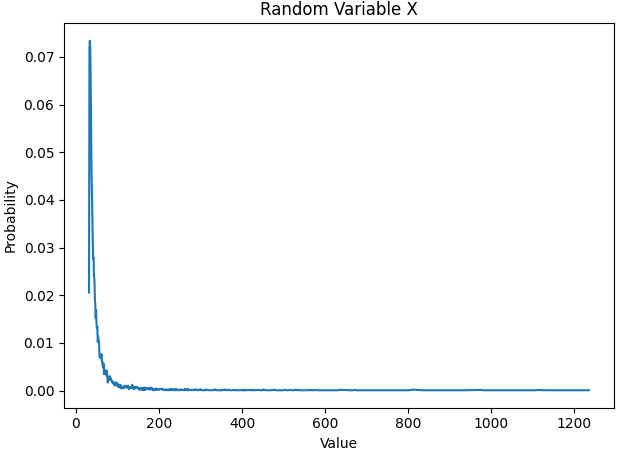
\includegraphics[scale=0.5]{graphs/random_variables/kakera}
  \caption{The kakera distribution. Large right skew---perfect for gamblers.}
\end{figure}

The data is of the form \( (X, p) \) as previously described. We now consider
the optimal rolling strategy, answering the question posed in the introduction,
\autoref{sec:intro}. Suppose we roll a character worth 100 kakera and we have
16 rolls left. Should we claim or continue rolling? The insight is that we can
assume the value of the 16 rolls is going to be the \textit{expected value}
of those rolls, which is true over a large number of samples. If we therefore
compute the expected value for 1 roll left, 2 rolls left, and so on until 30
rolls left, we can get cutoff values for each roll. If the expected value of
16 rolls is 120, then we should continue rolling. If the expected value is 80,
then we should claim the 100 kakera character and stop rolling. We now see how
to efficiently compute these expected values.

The overarching technique is known as \enquote{dynamic programming}, covered in
many \href{https://activities.tjhsst.edu/sct/otherlectures} {Senior Computer
Team} lectures. We need not give such a formal description, however, it is
simpler to describe the technique as \enquote{reducing the problem into smaller
subproblems}. Suppose we have 0 rolls left. Then the expected value is 0,
since we can't gain kakera if we can't roll. If we have 1 roll left, then the
expected value is just the expected value of the kakera random variable, which
we call \( X \). The interesting case comes in when we have 2 rolls left. Since
we know the value of 1 roll left is \( \E[X] \), then if we roll a character
greater than the cutoff, we keep it, and if we roll less than the cutoff, we
continue rolling and keep the \( \E[X] \) value of 1 roll left. Thus, the
expected value for 2 rolls is going to be a \enquote{capped} expected value sum
where the value of \( x \) is the maximum between \( x \) and the previously
computed value of having one less roll. If we call the random variable with
\( r \) rolls left \( X_r \), then we have a recurrence relation:
\[ \E[X_r] = \E[\max(X, \E[X_{r - 1}])] =
\sum_{x \in X} \max(x, \E[X_{r - 1}]) p(x) \]
Of course, for any recurrence relation we need a base case, and we already
found it: \( \E[X_0] = 0 \). It can be verified that the relation gives
\( \E[X_1] = \E[X] \) because we assume kakera values are necessarily positive.

We now use dynamic programming to compute these expected values quickly. If we
used the recurrence relation naively, to compute \( \E[X_r] \) we must do \( r
\) steps down to \( \E[X_0] \). However, note that in doing so we compute each
\( \E[X_0], \E[X_1], \dots, \E[X_r] \). Thus, if we repeatedly query \( \E[X_r]
\) (as we do while rolling), then we can store each intermediate result and
simply recall the stored value when the user requests it. This storage could be
done with a list, but is also elegantly done with Python's \texttt{lru\_cache}
from the \href{https://docs.python.org/3/library/functools.html}{functools}
module, a technique called \enquote{memoization}. We therefore do at most
\( r_\text{max} \) iterations of the expected value summation, where
\( r_\text{max} = 30 \).
\begin{algorithm}[H]
  \caption{Capped expected value}
  \label{alg:capped}
  \setlength{\partopsep}{-\topsep} % remove gap between top and bottom
  \begin{minted}[frame=none]{python}
  def capped(X: list, p: list, u: float) -> float:
      """ Returns E[X], but with the values capped at a minimum of u. """
      return E(p, X, lambda x: max(x, u))

  @lru_cache(maxsize=None)
  def Er(X: list, p: list, r: int) -> float:
      """ E[X_r], where X_r is X with possibly r more samples. """
      # if r = 0, then we're out of samples and has a constant value of 0
      return 0 if r <= 0 else capped(X, p, Er(i, r - 1))
  \end{minted}
\end{algorithm}

Finally, we show how to speedup the \texttt{capped} function. The observation
is that since the \( X \) list is sorted, there is some index \( i \) such that
every index less than \( i \) has a value less than or equal to \( \E[X_{r -
1}] \), and every index greater than or equal to \( i \) has a value greater
than \( \E[X_{r - 1}] \). We can therefore partition \( X \) into two halves
like in quicksort; in the left half we use the value \( \E[X_{r - 1}] \) and
in the right we use the original value:
\begin{align*}
  \sum^{i - 1}_{j = 0} \E[X_{r - 1}] p(x_j) &+ \sum^n_{j = i} x_j p(x_j) \\
  = \E[X_{r - 1}](p[0] + p[1] + \dots + p[i - 1]) &+ \sum^n_{j = i} x_j p(x_j)
\end{align*}
Notice that \( F[i] = p[0] + p[1] + \dots + p[i - 1] \) and that the right hand
side is simply a suffix sum of the expected value. We can therefore also run a
prefix sum on the expected value to efficiently calculate it, since the prefix
sum gives the sum between any two indexes.
\begin{minted}[label=fast capped]{python}
# expected value prefix sum
ev = prefix_sum([X[i]*p[i] for i in range(N)])

def capped(X: list, F: "cmf", prefix: list, u: float) -> float:
    """ Returns E[max(X, u)] in O(log n). """
    i = bisect.bisect(X, u)
    return u*F[i] + query(prefix, i, N - 1)
\end{minted}

The exact distinction of less than or equal to will not be relevant, since
if a value \( x \) is exactly equal to \( \E[X_{r - 1}] \), it does not matter
whether it goes into the left or right side. Our algorithm is now
\( O(\log n) \) per query of \texttt{Er} (amortized), so
\( O(r_\text{max} \log n) \) overall.

Armed with this algorithm, we can directly apply it to our data:
\begin{SCfigure}[1][h!]
  \centering
  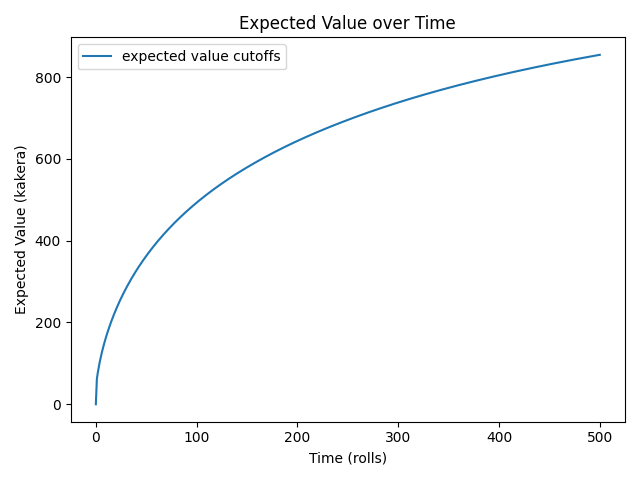
\includegraphics[scale=0.6]{graphs/expected_value/model.png}
  \caption{Expected value over increasing rolls.}
\end{SCfigure}

As expected, the expected value increases sharply in the beginning and
gradually levels off. It will asymptote at the maximum value, but takes many
rolls to reach that state (since the higher kakera characters are so rare).

\subsection{Batching}
Satisfied with our initial model, we now successively refine it. The
game I presented was a simplification; in reality one gets 10 rolls per
hour, and is able to claim any character within about a minute. Thus,
if someone rapidly runs \texttt{\$wa}, they can take their pick of any
of the 10 characters rolled. Assuming the goal is to maximize kakera,
they obviously take the maximum kakera value of those characters.

\subsubsection{Derivation of the Max of i.i.d. Random Variables}
The probability-theoretic question is as follows: what is the distribution of
the max of n independent and identically distributed (i.i.d.) random variables?
As is common in probability, the easiest way to find the PMF of a discrete
random variable is to first find the CDF of a continuous random variable.

Suppose the random variable \( X \) has CDF \( F(x) \) and PDF \( F'(x) =
f(x) \), and that the random variable \( Z = \max(X_1, X_2, \dots, X_n) \) is
the max of \( n \) samples of \( X \). We wish to find the CDF of \( Z \). By
definition, the CDF is the probability the random variable is less than or
equal to \( x \). If at least one of the random variables was greater than
\( x \), then the max would be greater. Therefore for the max of the random
variables to be less or equal to \( x \), they all have to be less than or
equal to \( x \). Since each has a CDF of \( F \) and they are independent,
the probability each is less than \( x \) is the product:
\[ p(X_1 \leq x, X_2 \leq x, \dots, X_n \leq x) =
  F(X_1) F(X_2) \dots F(X_n) = F(X)^n \]
To find the PDF, we can simply differentiate
with respect to \( x \), using the chain rule:
\[ g(x) = \frac{dF}{dx} = n F(X)^{n - 1} f(x) \]
where \( g(x) \) is the PDF of the random variable \( Z \).

We now apply the continuous derivation to the discrete case. While it
is true that \( G[i] = F[i]^n \) where \( G \) is the CMF of \( Z \)
and \( F \) is the CMF of \( X \), we cannot differentiate. We instead
use a \enquote{discrete derivative}, or subtract adjacent indexes of \(
G \) to recover the PMF \( g \). Since \( G[i] = g[0] + g[1] + \dots +
g[i - 1] \) and \( G[i + 1] = g[0] + g[1] + \dots + g[i] \), \( g[i] =
G[i + 1] - G[i] \). Lastly, we index \( Z \) by its \( n \), e.g. \(
Z_3 = \max(X_1, X_2, X_3) \). We therefore compute \( Z_1, Z_2, \dots,
Z_B \) where \( B = 10 \) since we get 10 rolls per \enquote{batch}.
\footnote{Yes, we can avoid the use of \texttt{pow} and shave a log factor
by using \( Z_{B - 1} \) to compute \( Z_B \) since \( Z_B[i] = F[i] Z_{B
- 1} [i] \). Since \( B = 10 \) is small, I show the simpler method.}
\begin{minted}[label=cmf of Z]{python}
Fzs = [[pow(v, b) for v in F] for b in range(B + 1)]
\end{minted}

As derived, the PMF of \( Z_b \) is the adjacent differences of the CMF. 
\begin{minted}[label=pmf of Z,frame=topline]{python}
def fz(z: float, b: int=B) -> float:
    """ pmf of Z. """
    return Fzs[b][D[z] + 1] - Fzs[b][D[z]]
\end{minted}

Note that while we use Python's builtin \texttt{pow} function, we could
implement fast exponentiation ourselves. We want to compute \( x^e \) where
\( x \) is a float and \( e \) is necessarily an integer. If we think of
the exponent \( e \) as a binary number, we can write \( x^e \) as the
product of \( x \) to the power of some powers of 2. The trick is that if
we repeatedly square \( x \), we get powers of 2, e.g. \( x^2, x^4, x^8,
\dots \). Thus, we can get to the highest set bit (most significant bit)
of \( e \) in \( O(\log e) \), and by keeping track of the powers we used
to get there we can therefore compute \( x^e \) in \( O(\log e) \). There
is no reason to use our function, however, since under the hood Python's
\texttt{pow} uses this technique for integer powers.
\begin{algorithm}[H]
  \caption{Fast exponentiation}
  \label{alg:exp}
  \setlength{\partopsep}{-\topsep} % remove gap between top and bottom
  \begin{minted}[frame=none]{python}
  def exp(b: int, e: int) -> int:
      """ Compute b^e in O(log e). """
      rtn = 1
      while e > 0:
          # if bit on in the binary representation of the exponent
          if e & 1 == 1:
              rtn *= b
          e >>= 1
          b *= b
      return rtn
  \end{minted}
\end{algorithm}

With the PMF of \( Z \) derived, we can visualize it with a graph:
\begin{figure}[h!]
  \centering
  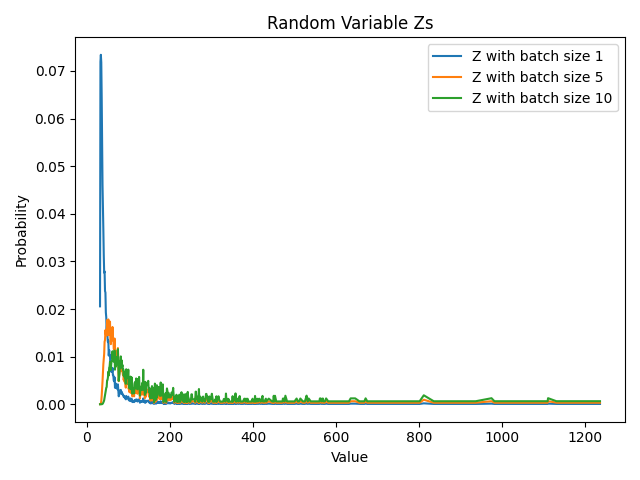
\includegraphics[scale=0.6]{graphs/random_variables/kakera_z.png}
  \caption{Random variables \( Z_5 \) and \( Z_{10} \) plotted against \( X \)}
\end{figure}

The effect of the max sharply decreases the peak of the PMF, instead
spreading out the probability mass over the right skew. In general,
the distribution is shifted to the right as expected; a larger batch
size will monotonically increase kakera value.

\subsubsection{Naive Implementation}
We now apply the derived PMF and CMF of \( Z \) to the original problem of
determining when to claim a character. Clearly, we can recycle our original
\hyperref[alg:capped]{capped expected value}. We simply substitute \( (Z_B,
p_{Z_B}) \) for \( (X, p) \) and change \( r_{\text{max}} \) to 3 since each
\enquote{roll} (sample of the random variable) is equivalent to 10 rolls.
\begin{SCfigure}[1][h!]
  \centering
  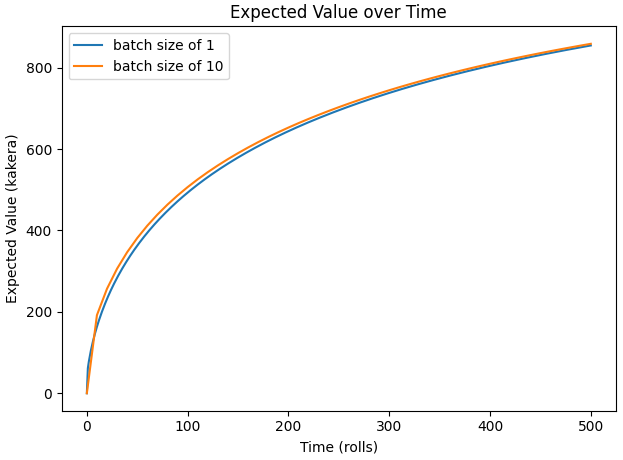
\includegraphics[scale=0.5]{graphs/expected_value/model_10}
  \caption{Batch size of 1 (previous model) versus batch size of 10.}
  \label{fig:batch}
\end{SCfigure}

As expected, the extra information provided by the ability to choose the
largest value out of a batch of 10 rolls yields a slight advantage over
immediately deciding whether or not to claim after a roll (which can be
thought of as a batch size of 1). This advantage decreases over time as
both curves asymptote.

There is one problem, however, and that is our new model only works for rolls
that are a multiple of 10 (since we can only move in samples of \( Z_{10}
\)). One notices in the graph that the orange starts \textit{under} the blue,
since it is at 0 for the first 10 rolls. This is a problem because people do
not necessarily roll in perfect batches of 10; one might hypothetically be too
slow or \enquote{sell} their rolls to other users after they have claimed,
letting another person claim from their now useless rolls (a practice analyzed
in \autoref{subsec:price}).

\subsubsection{Fractional Batching}
We now consider how to extend the previous \enquote{batched} model to any
number of rolls. If the number of rolls is not a multiple of 10, we simply use
\( Z_{r \% 10} \) instead of \( Z_{10} \), where \( \% \) is the 
\textit{modulo} operator, which gives the integer remainder
after dividing \( r \) by 10. If \( r \) is a multiple of 10,
then \( r \% 10 \) is 0 so we must explicitly default to \( Z_{10} \). 
\begin{algorithm}[H]
  \caption{Fractional batching model}
  \setlength{\partopsep}{-\topsep} % remove gap between top and bottom
  \begin{minted}[frame=none]{python}
  @lru_cache(maxsize=None)
  def Ef(r: int, b: int=B) -> float:
      """ E[X_r], where Z_r is extended to all r's. """
      n = r % b if r % b != 0 else b
      return 0 if r <= 0 else capped(Z, Fzs[n], evzs[n], Ef(r - n, b))
  \end{minted}
\end{algorithm}

In terms of notation, we denote the random variable with \( r \) rolls left
as \( X_r \), and \( \E[X_r] \) is now computed as shown above, instead of
the previous immediate decision method. Using this more general function, we
can correct \autoref{fig:batch}:
\begin{figure}[h!]
  \centering
  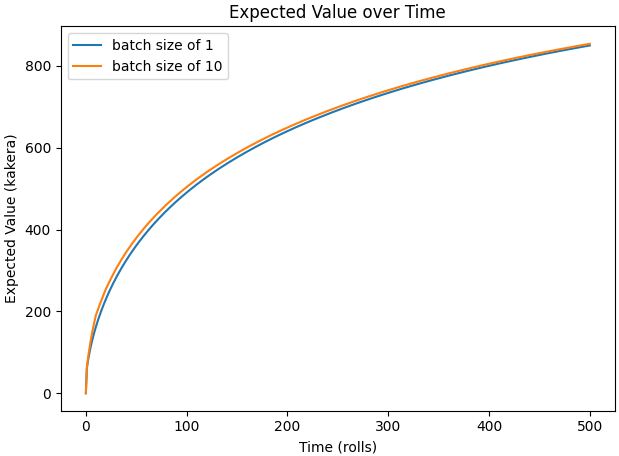
\includegraphics[scale=0.6]{graphs/expected_value/model_10f.png}
  \caption{Batched model adjusted for fractional batches.}
\end{figure}

While we are getting a feel for the model, we can also experiment
with changing the batch size while the number of rolls is fixed.
\begin{figure}[h!]
  \centering
  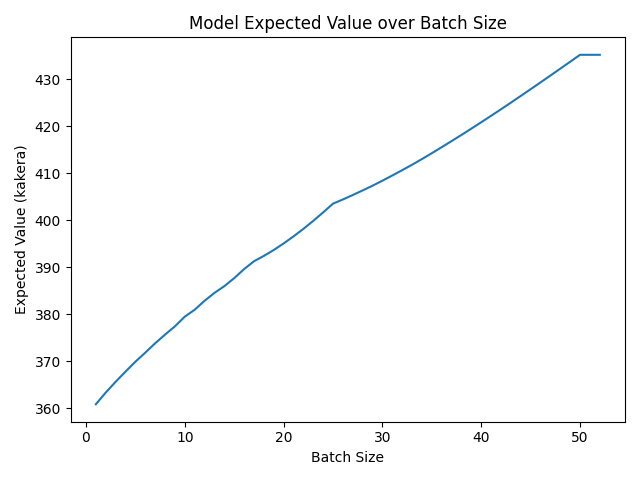
\includegraphics[scale=0.6]{graphs/expected_value/batch_size.png}
  \caption{Expected value over increasing batch size, \( r = 50 \).}
\end{figure}

As batch size increases, expected value increases seemingly
linearly. The flat part at the end is because the number of
rolls is 50, so a batch size greater than 50 has no effect.

\subsection{Putting it Together}
Satisfied with our model, we now create an agent which implements a concrete
rolling strategy according to our theoretical calculations. This will serve
three purposes: it is easier to work with from the perspective of an end user
since we are essentially creating an API, it will force us to somewhat simulate
the system so we can use this model for other downstream purposes, and finally
it will let us use code to test whether the math aligns with reality. Looking
towards the future, we will implement one last model in \autoref{subsec:rolls}
that is \textit{a posteriori}; its behavior depends in part on what one
actually rolls. Thus, we need an agent to model such behavior.

Our agent will take \( R \), the maximum number of rolls, and \( B \), the
batch size. Because it will frequently access the expected value cutoffs,
we pre-compute these values and store them. Finally, we will maintain all
instance variables in the \texttt{reset} function, which will allow us to
reset the game without needing to create a new object.
\begin{minted}[label=init method]{python}
class Model():

    """ Models interactions with the kakera random variable. """

    def __init__(self, R: int=prob.R, B: int=prob.B) -> None:
        self.R, self.B, self.offset = R, B, R % B
        # precompute list of expected values for each roll
        self.E = [prob.Ef(r, B) for r in range(R + 1)]
        self.reset()
\end{minted}

What attributes are specific to each game? We must know how many rolls we have
left, \( r \). If we are in the middle of a batch, we must know the kakera
values of the past characters rolled which we will store in a list \texttt{l}.
It is not strictly necessary but helpful to maintain the largest kakera value
seen so far in a batch, \( b \). Finally, to account for incomplete batches, we
assume that an incomplete batch will be the first to finish, and then the rest
of the batches are complete. Therefore we maintain the \texttt{size} variable,
which tells us how many values the current batch will hold. It is initially
\texttt{offset}, defined in \mintinline{python}{__init__} to be \( R \% B \),
and if \texttt{offset} is 0, it is the standard batch size \( B \).
\begin{minted}[label=reset method]{python}
def reset(self) -> None:
    """ Reset to the inital model. """
    # number of rolls left, list of seen kakera values, best value
    self.r, self.l, self.b = self.R, [], float("-inf")
    self.size = self.offset if self.offset > 0 else self.B
\end{minted}

The single method necessary for the operation of the model is \texttt{update},
which takes in a kakera value \( k \) that represents a roll. If the model
decides to claim, it returns the index of the value in the current batch it
wants to claim. Otherwise, it returns \mintinline{python}{None}.

We first determine whether or not the current batch has ended. If
it has, we reset \texttt{l} to a empty list, we set \( b \) to \(
-\infty \), and we set \texttt{size} to \( B \) (since we assume
the first batch is the one containing the one possible offset).

We then update the model's state with the new kakera value. We add \( k \) to
\texttt{l}, and set \( b \) to \( \max(b, k) \). We also decrement \( r \)
since we just used a roll.

With the bookkeeping finished, we are finally ready to determine whether or
not to claim this value (or any value in the current batch). As justified
in \autoref{sec:model}, we claim if our current value is larger than the
expected value of the number of rolls left, which is \( r \) since we
already decremented \( r \). Thus, we compare \( b \) to \( E[X_r] \).
However, for true optimality we need another condition. It never makes
sense to end a batch midway, since we can always finish the batch out and
then make a decision. This seems to contradict our algorithm, but it will
be resolved in \autoref{subsec:price}. In terms of the \texttt{update}
function, however, all that is important is that we only claim when the
current batch is over, when the length of \texttt{l} is \texttt{size}.

\begin{minted}[label=update method]{python}
def update(self, k: int) -> int:
    """ Returns an index if claiming, otherwise None. """
    # new batch, reset seen and b, the max of the samples we've seen
    if len(self.l) == self.size:
        self.l, self.b, self.size = [], -float("inf"), self.B
    # update variables with new information
    self.l.append(k)
    self.b = max(self.b, k)
    self.r -= 1

    # no need to stop early, wait until the batch is complete 
    if self.b > self.Ef(self.r) and len(self.l) == self.size:
        return self.l.index(self.b)
\end{minted}

\subsubsection{Simulation of Mudae}
With the model complete, we now work on simulating Mudae. Our function will be
very similar to the model, starting by calling \texttt{reset} on the model and
initializing its own variables, \texttt{l} to hold kakera values, and \( r \),
the number of rolls remaining, starts at \( r_{\text{max}} = 30 \). We define
\texttt{offset} as \( R \% B \) again, and initialize \texttt{size} identically
to the model, fulfilling the assumption that the offset is removed first.
\begin{minted}[label=simulate header, frame=topline]{python}
def simulate(m: model.Model=model.Model()) -> float:
    """ Simulates a game. """
    m.reset()
    l, r, offset = [], prob.R, prob.R % prob.B
    size = offset if offset > 0 else prob.B # remove the offset first
\end{minted}

We get a kakera value \( k \) from the kakera random variable \( X \) with
\hyperref[alg:sample]{\texttt{sample}}. We add \( k \) to our list and call
the model's \texttt{update} function, which returns an index \( i \) if it is
claiming, \mintinline{python}{None} otherwise. If \( i \) is an index, we make
sure it is valid and return the kakera value it corresponds to. Otherwise, we
continue and decrement \( r \) since we just simulated a roll cycle. Once we
run out of rolls, we return 0 since the model didn't claim.
\begin{minted}[label=body of simulate]{python}
    while r > 0:
        # new batch, reset seen and assume offset has been taken care of
        if len(l) == size:
            l, size = [], prob.B
        k = sample()
        l.append(k)
        i = m.update(k) # give kakera value to the model 
        if i is not None:
            assert 0 <= i < len(l), "model did not give a valid index"
            return l[i]
        r -= 1
    return 0 # model didn't claim, kakera value of 0
\end{minted}

We can now verify that our math is correct by repeatedly running
\texttt{simulate} for a large number of times, perhaps \( 10^6 \).
The expected value is then simply the average value, the sum of the
values \texttt{simulate} returns divided by the number of trials.
\begin{minted}[label=empirical expected
value via the law of large numbers]{python}
def E(X, iters: int=10**6) -> float:
    """ Expected value by repeatedly sampling a random variable. """
    return sum(X() for i in range(iters))/iters
\end{minted}

This confirms that the model expected value is 306.064, which is significantly
higher than the expected value of the kakera distribution, 61.702. It is lower
than \( E[X_{30}] \), which is 342.126. \( X_{30} \) corresponds to if one was
able to do all 30 rolls and then pick the highest value. Our model, only able
to do batches of 10, is surprisingly close, however.

\subsection{\texttt{\$rolls} Model} \label{subsec:rolls}
We arrive at the last consideration in our model, the command \texttt{\$rolls}.
\texttt{\$rolls} will reset the number of rolls in the current batch, giving
10 rolls if the user is currently out of rolls. However, the usage of
\texttt{\$rolls} is limited to once per day. Given that we can claim every
3 hours, and therefore claim 8 times a day, it follows that the model must
use \texttt{\$rolls} with less than a \( \frac{1}{8} = 12.5\%\) probability.
We separate our discussion into two parts: the first on simply implementing
this new command in our model and simulation, and the second on the optimal
determination of when to use the command.

\subsubsection{Implementation}
Recall that the model emits an index if it wants to claim,
\mintinline{python}{None} otherwise. We define the constant \( \texttt{ROLLS}
= -1 \) which the model returns if it wants to use \texttt{\$rolls}, so there
is no ambiguity between resetting and claiming (indexes are nonnegative
integers). We also define \texttt{ROLLS\_CYCLE} to be 8, the number of
claim cycles until the model receives a new usage of \texttt{\$rolls},
and \texttt{ROLLS\_F} to be the probability it uses \texttt{\$rolls}, \(
\frac{1}{\texttt{ROLLS\_CYCLE}} \). Finally, we assume the model only uses
\texttt{\$rolls} once per claim cycle. The actual game limits usage to once
per \textit{interval}, which is equivalent to a batch in our formulation.
\footnote{If this limitation did not exist, check
\autoref{subsec:general} in the appendix for an analysis.}
It very rarely makes sense to use \texttt{\$rolls} \textit{before} we
are actually out of rolls; we would have to anticipate that at least 2
straight batches are bad (10--0, the first usage of \texttt{\$rolls}).
\footnote{It can be shown that the best return from a second use of
\texttt{\$rolls} is when the rolls from 10--0 are as bad as possible; the
return is then \( \E[Z_{20}] - \E[Z_{10}] \approx 86 \). Comparing to the
worst return for one use of \texttt{\$rolls}, it can be shown that that occurs
at the highest value which triggers a usage of \texttt{\$rolls}, or 72. In
that case the difference is \( \E[\max(Z_{10}, 72)] - 72 \approx 122 \).
Because the best possible return for a second use is less the worst possible
return for one use, it is never worth it to use \texttt{\$rolls} twice.}

The first thing we define is a helper function adjusting the state
of the model after a use of \texttt{\$rolls}. Since \texttt{\$rolls}
\textit{resets} the current batch (not necessarily adding 10 rolls),
we first create two helpful methods for modulo arithmetic. Any number
\( x \) under \( \mod n \) can be written in the form \( qn + r \),
or as a multiple of \( n \) and a remainder. The remainder \( r \) is
the \textit{modulo} of \( x \), \( x \mod n \) or \( x \% n \).

When we reset a batch of size \( x \), we are essentially finding the smallest
multiple of the batch size \( B \) that is greater than \( x \). To find the
largest multiple of \( B \) that is \textit{smaller} than \( x \), since \( x
\) can be written as \( qB + r \), the lower bound is just \( qB \). The upper
bound is thus \( qB + B \) or \( (qB + r) + (B - r) = x + (-x \mod B) \). Since
\( B - r \) is between \( 1 \) and \( B - 1\) if \( r \) is nonzero, \( B - r
= B - r \mod B = -r \mod B = -x \mod B \). If \( r = 0 \), then \( x \) is a
multiple of \( B \) and is its own lower and upper bound, \( -x \mod B = 0 \).

\begin{minted}{python}
def lower(x: int, b: int=B) -> int:
    """ Returns the  largest value n such that n <= r and n % B == 0. """
    return x - (x % b)

def upper(x: int, b: int=B) -> int:
    """ Returns the smallest value n such that n >= r and n % B == 0. """
    return x + (-x % b)
\end{minted}

If we use \texttt{\$rolls}, the amount of rolls we gain is the upper bound of
\( r + 1 \), since if \( r \) is a multiple of \( B \) we want it to reset
to the higher multiple of \( B \), not at its own value. We set \( \Delta =
\texttt{upper}(r) - r \), and update \( r \) to \( r + \Delta \) to put it at
its new value. We update \texttt{size} as well to \( \texttt{size} + \Delta
\), because our batch now contains the characters currently in the batch along
with the new characters we roll from the rolls we got from \texttt{\$rolls}
(assuming we do all our rolls within the minute long grace period). Finally,
since we only use one \texttt{\$rolls} per claim, we set \texttt{rolls\_use}
to \mintinline{python}{False}, barring future usage of \texttt{\$rolls}.

\begin{minted}[label=helper function after using \$rolls]{python}
def rolls(self) -> None:
    """ Update the model's parameters if it uses $rolls. """
    delta = prob.upper(self.r + 1, self.B) - self.r
    self.r += delta
    self.size += delta
    self.rolls_use = False
\end{minted}

With the model adjusted, we now focus our attention on the simulation.
We first need to give rolls to the model, which we will store in the
\texttt{rolls\_left} instance variable. We could give the model a roll with
\( \frac{1}{8} \) probability, but it is more consistent and accurate to
the game to simply give the \texttt{simulate} method an integer tracking
the game number, and give a usage if the index is a multiple of 8.
\begin{minted}[label=new simulate header]{python}
def simulate(m: model.Model=model.Model(), index: int=0) -> float:
    """ Simulates a game. """
    m.reset()
    # give the model a roll every ROLLS_CYCLE claim iterations
    if model.ROLLS_AVAILABLE and index % model.ROLLS_CYCLE == 0:
        m.rolls_left += 1
    ...
\end{minted}

The only other change to make is when handling output from the model. If the
output is not \mintinline{python}{None}, we know that the model is performing
an action and handle the action appropriately. Claiming is handled the same,
and we handle \texttt{\$rolls} according to the \texttt{rolls} method defined
above for the model.
\begin{minted}[label=new simulate body]{python}
    ...
    i = m.update(k) # give kakera value to the model 
    if i is not None:
        if i == model.ROLLS:
            assert model.ROLLS_AVAILABLE, "$rolls is not allowed"
            assert m.rolls_left > 0, "model doesn't have available rolls"
            # $rolls resets the batch instead of adding the batch size
            delta = prob.upper(r, prob.B) - r + 1
            r += delta
            size += delta
            m.rolls_left -= 1
        else:
            assert 0 <= i < len(l), "model did not give a valid index"
            return l[i]
    ...
\end{minted}

\subsubsection{Optimization}
With the framework of \texttt{\$rolls} complete, we now discuss the
determination of when to use the command. Very simply, optimization
problems are always determined by two things: what we want to optimize
and what the constraints are. The constraint is that we can only use
\texttt{\$rolls} every one in 8 claim cycles. We want to optimize kakera,
so we should use our limited number of \texttt{\$rolls} on the situations
that maximize the gained value. This is equivalent to being in the
\textit{worst} situations---the worse the situation, the more advantage
additional rolls gives us (put another way---the better the situation,
the less probability \texttt{\$rolls} can improve on the situation).

Going from the abstract to the more specific, the measure of the quality
of a situation is simply its kakera value. If we're about to claim a low
kakera value character, that is a situation to avoid. So we should use
\texttt{\$rolls} for any kakera value less or equal to a certain cutoff,
\( k^* \). How should \( k^* \) be determined? Well, suppose we have the
CMF of the model, \( F_\text{model}(k) \), which gives the probability we
claim a value less than or equal to \( k \). Because we use \texttt{\$rolls}
whenever we're about to claim a value less than or equal to \( k^* \), the
probability we use \texttt{\$rolls} is \( F_\text{model}(k^*) \), which must
be \( \leq \frac{1}{8} \). Therefore, we need to compute \( F_\text{model}
\) in order to compute \( k^* \).

In order to compute \( F_\text{model} \), we first need to compute the
probability of emitting a value at a particular number of rolls left \( r \),
\( p(\text{emit at } r) \). To compute that, we first need to compute its
CMF, \( p(\text{emit at} \leq r) \). I know, very straightforward. Suppose we
know the probability of getting to \( r + 1 \) rolls left is \( F(r + 1) \).
Then the probability of getting to \( r \) rolls left is if we don't emit at
roll \( r + 1 \). We don't emit if the value rolled is less than the expected
value cutoff, or if \( Z_B \leq \E[X_{r}] \). By definition, \( p(Z_{B} \leq
\E[X_{r}]) \) is the CMF of \( Z_B \), a value we'll call \( p \). So \( F(r)
= p F(r + 1) \), and the base case is that \( F(30) = 1 \) (since the largest
number of rolls we have is 30). Note that if \( r \) is not a multiple of the
batch size, \( p = 1 \) since we only claim at the end of a batch.

In order to implement this, we first define a useful function which gives
the current \( Z_n \) (since if the number of rolls isn't a multiple of the
batch size, we'll have partial batches). We use \( Z_B \) by default, but
if we're in the offset (if \( r \geq R - \text{offset} \)) then we use \(
Z_{\text{offset}} \).
\begin{minted}[label=current random variable]{python}
def __Z(self, r: int) -> list:
    """ Returns the correct cmf of Z_n, accounting for offset. """
    return prob.Fzs[self.offset if r >= self.R - self.offset else self.B]
\end{minted}

The CMF then follows from the discussion above and
the PMF is simply the adjacent difference of the CMF.
\begin{minted}[label=cmf and pmf of emitting a value at r rolls left]{python}
def F_r(self, r: int) -> float:
    """ Probability of getting to roll r. """
    # since we never claim in the middle of the batch, use Z instead of X  
    p = prob.cmf(self.__Z(r), self.Ef(r)) if r % self.B == 0 else 1
    return 1 if r == self.R else p*self.F_r(r + 1)

def p_r(self, r: int) -> float:
    """ Probability of emitting a value at roll r, pmf of F_r. """
    return self.F_r(r) - self.F_r(r - 1)
\end{minted}

We now compute the probability of emitting a kakera value \( k \). We
can do casework on each possible number of rolls left \( r \) thanks
to conditional probability, a quick description of which is given in
the appendix, \autoref{subsec:conditional}.
\[ p(\text{emit value } k) = \sum^R_{r = 0} p(k|r) \cdot p(r) \]
\( p(r) \) is the function defined above and \( p(k|r) \) is simply the
probability we emit \( k \) given we have \( r \) rolls left. We emit if we
roll a value \textit{higher} than the cutoff, so the denominator will be the
survival function while the probability we emit \( k \) is the PMF, assuming \(
k \) is greater than the cutoff. If it isn't, \( k \) has a probability of 0.
\[ p(k|r) = \frac{p_{Z_B}(k)}{1 - F_{Z_B}(\E[r])} \]

Rewriting \( p(\text{emit value } k) \) using \( p(k|r) \), 
\[ p(k) = p_{Z_B}(k) \sum^R_{r = 0} \frac{p(r)}{1 - F_{Z_B}(\E[r])} \] 

Note that the sum is a function of \( r \) and not \( k \), so it can
be cached for different \( k \). But we can't just store the right sum
as a scalar because if \( k \) is less than the cutoff at a particular
level, its probability is zeroed out. We therefore store the prefix sum
and binary search on the cutoffs to find the level \( r' \) such that \(
k \geq \E[X_{r'}] \). We also need to account for a possible offset by
switching \( p_{Z_B} \), so we in fact maintain two prefix sums, one for
\( r \) below the offset and the other for \( r \) above the offset.
\begin{minted}[label=calculating the pmf of emitting a value k]{python}
def __cache_p_k(self) -> None:
    """ Generate cache for p_k """
    self.poss = [1 - prob.cmf(self.__Z(r), self.Ef(r))
                  for r in range(self.R)]
    i, f = self.R - self.offset, lambda r: self.p_r(r + 1)/self.poss[r]
    self.cond = prob.prefix_sum(list(map(f, range(i))) + [0]*self.offset)
    self.coff = prob.prefix_sum([0]*i + list(map(f, range(i, self.R))))

@lru_cache(maxsize=None)
def __p_k(self, k: int) -> float:
    """ Probability of emitting the kakera value k. """
    i = min(bisect.bisect(self.E, k), self.R)
    return self.fz(k)*self.cond[i] + prob.fz(k, self.offset)*self.coff[i]
\end{minted}

With \( p(k) \) computed, we now have \( F_\text{model} \) which if you will
recall, we use to find the largest value \( k^* \) such that we will use
\texttt{\$rolls} if we're about to claim a value \( \leq k^* \). We simply
binary search on the CMF to find the value with CMF greater than \( \frac{1}{8}
\), and subtract 2 (one for the CMF, and one to make it less than).
\begin{minted}[label=the rolls model]{python}
def __init__(self, R: int=prob.R, B: int=prob.B,
  ...
  if ROLLS_AVAILABLE:
      # generate cmf of p_k
      self.Fk = prob.prefix_sum(list(map(self.__p_k, prob.X)))
      # the largest value k* such that Fk(k*) triggers the roll cutoff
      self.kp = prob.X[bisect.bisect(self.Fk, ROLLS_F) - 2]
      assert prob.cmf(self.Fk, self.kp) <= ROLLS_F, "valid cutoff"
      self.rolls_left = 0

def update(self, k: int) -> int:
    ...
    # no need to stop early, wait until the batch is complete 
    if self.b > self.Ef(self.r) and len(self.l) == self.size:
        # use $rolls if emitting this bad of a value has probability 1/8
        if self.rolls_use and self.rolls_left > 0 and self.b <= self.kp:
            self.rolls()
            return ROLLS
        return self.l.index(self.b)
\end{minted}

Finally, we can recompute the PMF for the rolls model, since using rolls will
change the behavior of our model. To simplify the calculations, we assume
that \( k^* \leq \E[X_B] \), an assumption which can be checked empirically.
Intuitively, the more \texttt{\$rolls} we get, the larger \( k^* \) will be
since we can use it more, and the less uses we get the smaller \( k^* \) will
be. \( \frac{1}{8} \) is sufficiently small to force \( k^* \leq \E[X_B] \),
which means that we only use \texttt{\$rolls} with no rolls left (\( \E \) is
monotonically increasing with the number of rolls left, therefore for a larger
number of rolls left, if we claimed, we must have claimed for a value \( > k^*
\)). Thus, the PMF is only different for the last layer. We therefore look at
\( p_{\text{last}}(k) \), the probability of emitting the kakera value \( k
\) at the last layer. The old PMF was simply \( Z_B \). For the new PMF, we
sample \( Z_B \) once. If the value is \( \leq k^* \), we sample \( Z_B \)
again. We now analyze two cases, \( k > k^* \) or \( k \leq k^* \) which are
independent and cover all cases.

Let's say we're looking at a value \( k > k^* \). Then we could have rolled it
in the initial sample and stopped, or the first sample was \( \leq k^* \), so
we did a second sample and rolled \( k \). Since the cases are independent, we
add their probabilities:
\[ p_{Z_B}(k) + F_{Z_B}(k^*) p_{Z_B}(k) = (1 + F_{Z_B}(k^*)) p_{Z_B}(k) \] 

In the case that \( k \leq k^* \), we must have that \( k \) is the largest
value in two separate samples of \( Z_B \), or simply the largest sample of
\( Z_{2B} \). Thus, the probability is \( p_{Z_{2B}}(k) \).
\begin{minted}[label=last layer pmf of the rolls model]{python}
def p_last(self, k: int) -> float:
    """ Probability of emtting the kakera value k on the last layer. """
    return (1 + prob.cmf(self.Fz, self.kp))*self.fz(k) if k > self.kp \
            else prob.fz(k, 2*self.B)
\end{minted}

We now compute the overall PMF by simply swapping out the last layer PMF.
\[ p_\text{new}(k) = p(k) + p(\text{emit at layer 1})
  (p_\text{last}(k) - p_{Z_B}(k)) \]
\begin{minted}[label=pmf of the rolls model]{python}
def __rolls_p_k(self, k: int) -> float:
    """ Probability of emitting the kakera value k. """
    return self.__p_k(k) + self.p_r(1)*(self.p_last(k) - self.fz(k))
\end{minted}

With the mathematical analysis of the rolls model complete, we switch to a
quantitative and qualitative evaluation. Starting with the expected value: 
\begin{table}[h!]
  \centering
  \begin{tabular}{|c|c|c|} 
    \hline
    Name & Expected value (kakera) & Standard deviation (kakera) \\
    \hline \hline
          Kakera &  61.702 &  79.727 \\ \hline
    \( Z_{10} \) & 191.873 & 196.072 \\ \hline
    \( Z_{30} \) & 342.126 & 259.412 \\ \hline
           Model & 306.064 & 255.263 \\ \hline
     Rolls Model & 322.036 & 252.524 \\ \hline
  \end{tabular}
  \caption{Table of random variables.}
\end{table}

Unsurprisingly, the expected value of the rolls model is
slightly higher, since it's sometimes able to avoid low
kakera values. Looking at the graphs confirms this trend.
\begin{figure}[h!]
    \centering
    \begin{subfigure}[h]{0.45 \textwidth}
      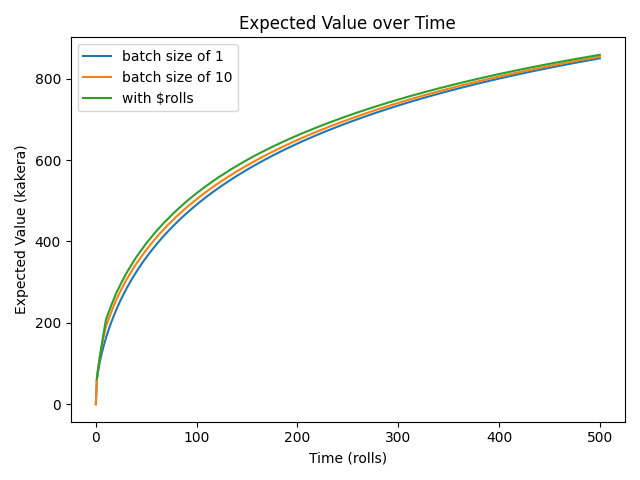
\includegraphics[scale=0.4]{graphs/expected_value/model_rolls.png}
      \caption{Expected value over rolls left.}
    \end{subfigure}
    \begin{subfigure}[h]{0.45 \textwidth}
      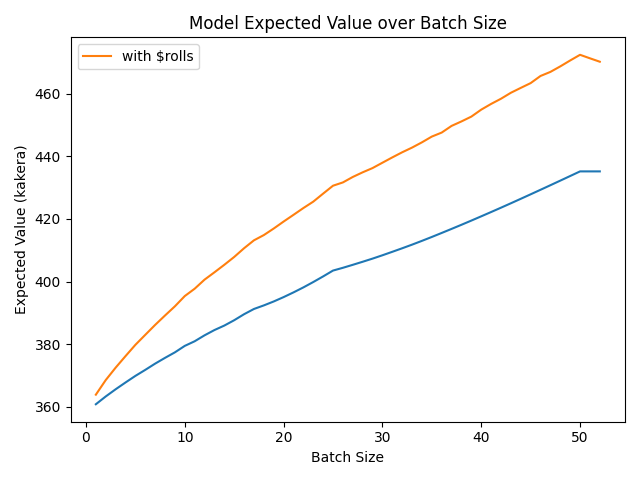
\includegraphics[scale=0.4]{graphs/expected_value/batch_size_rolls.png}
      \caption{Expected value over batch size.}
    \end{subfigure}
    \caption{Expected value graphs.}
\end{figure}

Since we have the PMF, we can now graph the model PMFs:
\begin{figure}[h!]
  \centering
  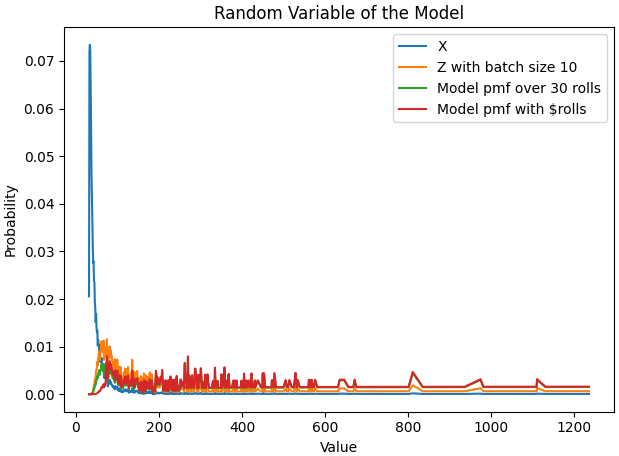
\includegraphics[scale=0.7]{graphs/random_variables/model_rolls.png}
  \caption{Model PMFs}
\end{figure}
Towards the left side, the rolls model has a much lower slope before rising
parabolically upwards because it is able to reduce the probability of low
kakera values. One interesting observation is that the local maxima in the
original distribution are magnified: see the spikes at 700, 800, 1000, and
1100. With the PMFs we can also analytically calculate the variance:
\begin{figure}[h!]
  \centering
  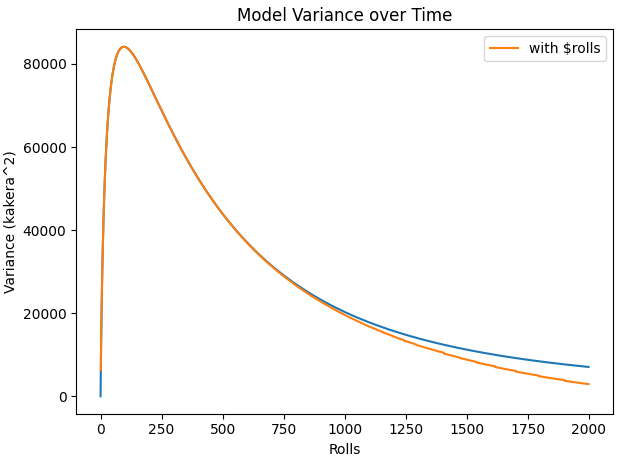
\includegraphics[scale=0.6]{graphs/variance/model_rolls.png}
  \caption{Variance over rolls left.}
\end{figure}

This has a surprisingly beautiful shape, coming up to a local maxima
before smoothly asymptotically approaching zero. The variance decreases
because more rolls essentially means more samples, but I'm not sure
why the variance increases towards the beginning. Whatever the case,
it sort of resembles a blackbody radiation curve so there may be some
connection to statistical thermodynamics.

Finally, we can graph variance over batch size:
\begin{figure}[h!]
  \centering
  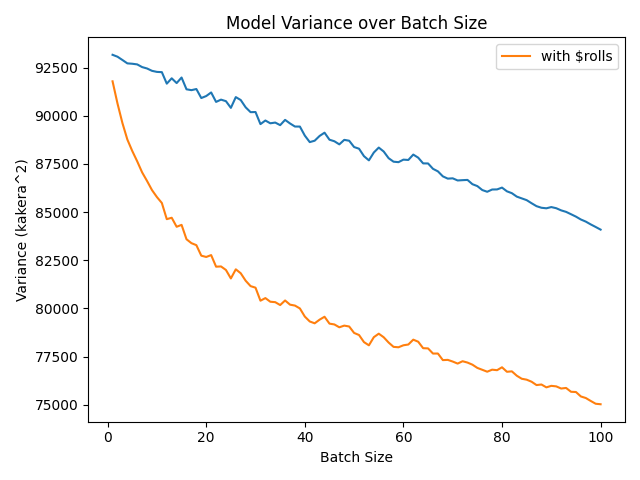
\includegraphics[scale=0.6]{graphs/variance/batch_size_rolls.png}
  \caption{Variance over batch size.}
\end{figure}

Without rolls the variance is suspiciously linear, which is quite surprisingly
for such a nonlinear model. With rolls the variance starts to curve, exposing
the underlying nonlinearity. Why increasing batch size has a seemingly linear
effect on both expected value and variance when the PMF changes with respect
to the power of the batch size is hard to determine. With the rolls model
complete, we now analyze one last mechanic.

\subsection{Roll Pricing} \label{subsec:price}
Recall we only claim at the end of a batch, never in the middle of a batch.
Doesn't this contradict our maxim \enquote{Claim when the current value is
greater than the expected value of \( r \) rolls left}? Well, what principle
justified our maxim in the first place? We have two options, claim or continue
rolling. If we claim, the value is the value of the character. If we continue
rolling, the value is the expected value of \( r \) rolls left. We want to
maximize value, so we pick the option which gives the larger value. But hold on
a second --- we have more specific information than just \( r \) rolls left!
In particular, if we're in the middle of the batch then we have some largest
value \( k \). The value of our current batch is then lower bounded by \( k
\). Thus, the value of continuing the batch is a capped expected value, \(
\E[\max(Z_n, k)] \) where \( Z_n \) is the appropriate batch random variable
and \( k \) is the current largest value in the batch, since if we roll values
lower than \( k \) we can always claim \( k \).
\begin{minted}[label=expected value of continuing]{python}
def Eloss(self, r: int, k: int) -> float:
    """ Expected value if the current batch is continued. """
    n = r % self.B
    return prob.capped(prob.Z, prob.Fzs[n], prob.evzs[n], k)
\end{minted}

The real value of our current state, or our \enquote{status quo} is then
the maximum between \( \E_{\text{loss}} \) and \( \E[X_r] \), since we
either claim in the current batch, or do our \( r \) remaining rolls.
\begin{minted}{python}
    def status_quo(self, r: int, k: int) -> float:
        """ Represents the current value. """
        return max(self.Eloss(r, k), self.Ef(r))
\end{minted}

We could therefore rewrite the rule of \enquote{claim when the value is greater
than the expected value and only when the batch is over} as \enquote{claim when
the value is greater or equal to the status quo}. If we're in the middle of a
batch, \( \E_{\text{loss}} \) is greater than \( k \), so we're never going
to claim\footnote{If \( k \) is the largest possible value, then the capped
expected value will not add to its value, so we would claim \( k \) immediately
instead of finishing the batch --- it's not possible to improve.}. If we're at
the end of a batch, then \( r \% B \) is 0, \( \E[\max(Z_0, k)] = k \) so \(
\E_{\text{loss}} \) reduces to \( k \), so checking whether \( k \) is greater
than the status quo reduces to checking whether \( k \) is greater than \(
\E[X_r] \). Why did we derive this alternative representation of our current
value when our more computationally efficient stopping rule works just fine?

We can now define \textit{opportunity cost}, the basis of value I will use to
justify the formulation of judging the value of buying or selling rolls. Since
other users are also on our Discord server playing Mudae, we can choose to buy
or sell rolls. Suppose we used all our rolls and didn't get a good value. Then
we can pay someone else to roll for us, and claim from their rolls. Suppose we
claim a high value character, and have rolls left. Then we can sell our rolls
to someone else, and let them claim from the rolls that are now useless to us.
How should buying and selling be priced?

We first analyze buying. If we buy \( b \) rolls, then our new expected value
is \( \E[X_{r + b}] \) compared to \( \E[X_r] \). If we were at a new batch
then the price at which we should buy these \( b \) rolls would simply be \(
\E[X_{r + b}] - \E[X_r] \) since we gain that much expected value from using
the \( b \) rolls. However, if we're in the middle of a batch we must use the
derived status quo calculation. If our status quo is more valuable than \(
\E[X_{r + b}] \) then the extra rolls don't hurt---we should price them at 0.
\begin{minted}[label=buy price]{python}
def __buy(self, r: int, k: int, b: int) -> float:
    """ Finds the price which we are indifferent to buying b rolls. """
    return max(self.Ef(r + b) - self.status_quo(r, k), 0)
\end{minted}

Selling is very similar. If we sell, then we must claim immediately, so our
current value is \( k \), the largest value in the current batch. If we didn't
sell, then the value would be the status quo. This elegantly accounts for
the case where the value of the status quo is \( k \), in which case we are
indifferent to selling and price our sales at \( 0 \).
\begin{minted}[label=sell price]{python}
def __sell(self, r: int, k: int) -> float:
    """ Finds the price which we are indifferent to selling r rolls. """
    return self.status_quo(r, k) - k
\end{minted}

In order to visualize the pricing for buying and selling, we assume we're
at a start of a new batch. In that case the value of buying is simply \(
\E[X_{r + b}] - \E[X_r] \). If we're buying one roll, then this is simply
the adjacent differences of the expected value graph.
\begin{figure}[h!]
  \centering
  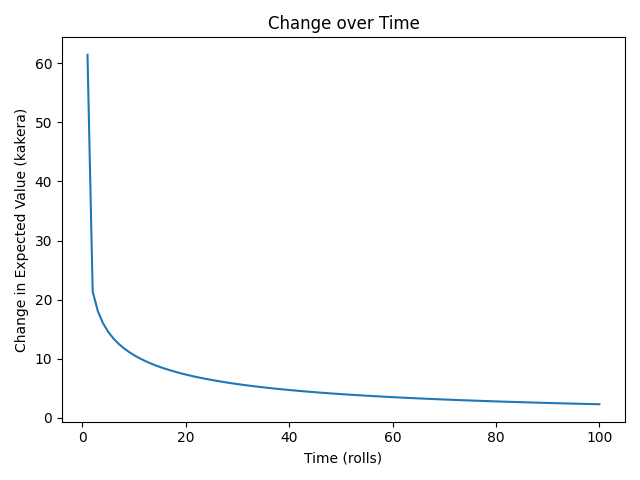
\includegraphics[scale=0.7]{images/graphs/deriv.png}
  \caption{Discrete derivative of the expected value graph.}
\end{figure}

The value of buying a single roll sharply
drops as the number of rolls left increases.

\section{Convolutions and the Central Limit Theorem}
\textit{This section is a mathematical tangent, feel free
to skip to the \hyperref[subsec:conclusion]{conclusion}.}

Suppose we know that we will do 5 claim cycles. By the linearity of
expected value, the expected value will be 5 times the expected value of
one claim cycle, but can we figure out the PMF of the new random variable?

\subsection{Derivation of the Sum of i.i.d Random Variables}

We have two independently and identically distributed random variables \( X
\) and \( Y \) and wish to find the PMF. Surprisingly enough, we can directly
compute the PMF without any CMF or continuous trickery. Suppose we want the
probability of the value \( v \) occurring. Then we can split into cases based
off \( X \)'s values. If \( X \) takes on some value \( i \) then \( Y \) must
take on the value \( v - i \) for the value of \( X \) plus the value of \( Y
\) to be v. Since \( X \) and \( Y \) are independent, the probability of them
taking their respective values is simply the product of the probabilities, and
we sum over all possible values of \( i \).
\[ p_{X + Y}(v) = \sum^{\infty}_{i = -\infty} p_X(i) p_Y(v - i) \]
We call this function the \emphasis{convolution} of the
PMFs \( p_X \) and \( p_Y \), denoted \( p_X * p_Y \).
\begin{theorem}
  The discrete convolution is equivalent to polynomial multiplication.
\end{theorem}
\begin{proof}
  We assume the discrete random variables takes on nonnegative integer values.

  We encode a random variable \( X \) into a polynomial \( a \) using the
  following: First, we represent polynomials as a coefficient list. For
  each value \( X \) can take, we index \( a \) at that value and put the
  probability it occurs at that index. Put another way, if \( x \) is a value
  of \( X \) occurring with probability \( p \), then we make \( a[x] = p \).

  If \( a \) and \( b \) are polynomial representations of \( X \) and \( Y
  \), then the convolution is: \[ (a * b)[n] = \sum^n_{i = 0} a[i] b[n - i] \]
  This is equivalent to the polynomial multiplication of \( a \) and \( b \).
\end{proof}

Along with computing the probability function of the sum of
two random variables, the convolution has many, many uses:
\begin{itemize}
  \item Signal processing,
    \href{https://www.ee.columbia.edu/~dpwe/papers/Wang03-shazam.pdf}{audio
    processing} (\href{https://arxiv.org/abs/1609.03499}{spectrograms})
  \item Polynomial multiplication,
    \href{https://hal.archives-ouvertes.fr/hal-02070778/document}{integer
    multiplication}
  \item \href{http://nablab.rice.edu/publications/JoA2005.pdf}{String matching}
  \item Differential equations: the Laplace transform of
  the convolution is the product of the Laplace transforms,
  \( \mathcal{L}\{f * g\} = \mathcal{L}\{f\} \mathcal{L}\{g\} \)
  \item \href{https://arxiv.org/abs/1911.06465}{Deepfake detection} (really!)
  \item Kernels in image processing 
  \item Gives \enquote{convolutional} neural networks their name
\end{itemize}

We do not discuss how to compute the convolution quickly; I have a 
\href{https://activities.tjhsst.edu/sct/lectures/2021/2020_10_23_FFT_handout.pdf}{lecture}.
It can be done in \( O(n \log n) \) with the Fast Fourier Transform
(FFT), compared to the naive polynomial multiplication of \( O(n^2)
\). Instead, we simply apply the convolution to compute the PMF of
the sum of i.i.d. random variables.

\subsection{The Central Limit Theorem}

The central limit theorem is one of the most surprising theorems in
probability; it states that the distribution of the average value of
multiple samples of a random variable approaches a normal distribution
as the sample size approaches infinity, for any random variable.

As proved previously, the sum of i.i.d random variables is the product of
their polynomial forms. Since each random variable has the same polynomial
form, it is the power of the polynomial. One could use a generalization of
the binomial formula, the multinomial coefficients to compute this power,
but it is simplest to use the \hyperref[alg:exp]{fast exponentiation} trick,
for \( \log k \) multiplications, using the convolution for each polynomial
multiplication. This yields a \( O(kn \log kn) \) time algorithm where \(
k \) is the number of samples and \( n \) is the length of the polynomial,
compared to \( O(k^2 n \log kn) \) without fast exponentiation and \( O(k^2
n^2) \) without either trick. The lower bound is \( O(kn) \).

We can directly apply this onto the PMF of the kakera distribution:
\begin{figure}[h!]
  \centering
  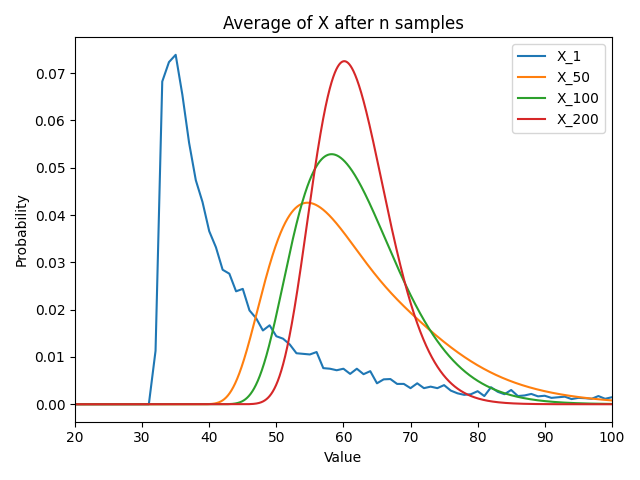
\includegraphics[scale=0.8]{images/graphs/clt.png}
  \caption{A demonstration of the central limit theorem.}
\end{figure}

As the number of samples increases, the graph becomes more normal. We see the
long right tail disappear as the PMF becomes more symmetric, the rightness
being absorbed in the peak shifting to the right. The variance also lowers, as
the graph becomes tighter and the peak grows higher. The peak will eventually
reach the expected value of the distribution, 61.702 while the graph becomes
narrower and narrower.

\section{Is the Model Realistic? \enquote{Optimal}?} \label{subsec:conclusion}
Throughout this paper, we have been focused on maximizing expected
value. I claim that the model is optimal with respect to its expected
value. But is expected value really the thing we want to maximize?

Suppose I offer you a 50\% chance to get a million dollars versus a
80\% chance for \$500,000. Which should you pick? Despite the higher
expected value for the million dollars, it is not obvious. One can
argue the difficulty is psychological in nature or related to the
diminishing utility of money rather than the pure mathematically
\enquote{rational} action to take. But it is hard to separate.

Because of the strong law of large numbers, taking the average of many samples
of a random variable will converge to the expected value, as the number of
samples approaches infinity. Expected value is then essentially the value
over an infinite \textit{timescale} or \textit{horizon}. Generally speaking,
the lower the variance, the faster the average value will converge to the
expected value. But even if the variance is infinite it will still converge.
Is our timescale really infinite in the real world? Are we going to play this
Discord game forever? The timescale really does matter, and with it what we
define as \enquote{optimal}.

For example, take the
\href{https://plato.stanford.edu/entries/paradox-stpetersburg/}{St.
Petersburg paradox}. The expected value of the game is infinite, but if we
pay \$50 we have only about a 3\% chance to get our money back. If we play
the game \textit{infinite} times, yes, the expected value will converge
to infinity. But if we play only once or twice, should we really sell
everything we own and take out loans for the opportunity to play this game?
The St. Petersburg paradox poses a fundamental threat to the notion that
maximizing expected value is the \enquote{rational} thing to do.

One way to fix this it to notice that if we don't know the rules of the
game and need to figure them out as we play, then we don't know what hasn't
happened --- events with low probability aren't likely to happen, so we
won't even know they exist. If we only play once or twice, we might guess
that the expected value is around 4. So one rule would be \enquote{disregard
low probability events}. This elegantly works if we play the game multiple
times, since the more times we play the game the more likely low probability
events are to occur, which might move us over the arbitrary \enquote{low
probability} cutoff. But there is a clear weakness: suppose we disregard
any events with a probability \( \alpha = 0.05 \) or lower. I now offer you
the following game: I give you a million dollars, except I also hand you a
slip of paper with a number between 1 and 20 written on it. The chance that
any particular situation occurs is \( \frac{1}{20} \leq \alpha \). So you
conclude the value of the game is 0 since no situations occur! If I wrote
a real number on the slip of paper, then no \( \alpha \) is low enough. So
disregarding low probability events is clearly not a general principle.

Well, instead of comparing values what if we duel the two strategies? We
compare the strategy of \enquote{don't play the game} versus the strategy of
\enquote{play the game at some cost} and simply pick the one that is more
likely to win. But this also has a clear failure point --- it doesn't account
for the \textit{magnitude} of a win. I offer you a 100\% chance for 1 dollar
versus a 49\% chance for 1 million dollars. Let's say I take the dollar while
my friend aims for the million dollars. The chance I beat my friend is going
to be 51\% while the chance my friend beats me is 49\%. I am clearly more
likely to win, so I should take the dollar! Of course, while the million
dollars is slightly less likely, it gives a much larger reward when it does
happen. So comparing strategies naively is also not a general principle.

\label{here}
Let us conclude by going back to Mudae. We have spent \pageref{here}
pages describing exactly how to maximize expected value, only to just now
question the entire basis of our modeling. It is to temper expectations.
Many people have told me that the model is too optimistic and is not
aligned with the reality of the game. I sometimes feel the same way
myself. Ignoring psychological and irrational explanations, one reason is
that expected value is not a perfect metric. But it is good enough.
\begin{figure}[h!]
  \centering
  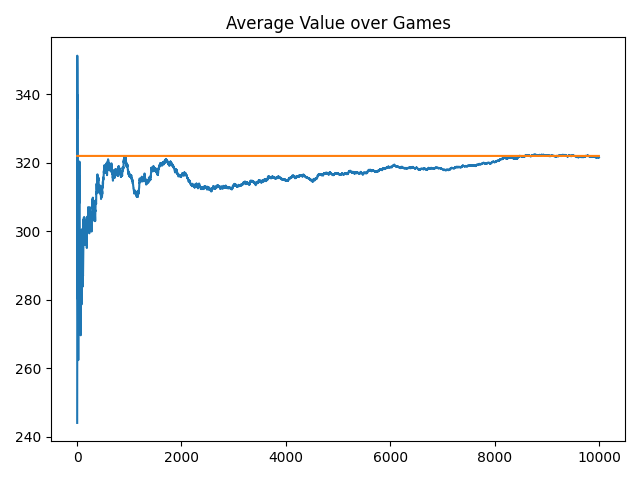
\includegraphics[scale=0.6]{graphs/game_value.png}
  \caption{Average value over number of games.}
\end{figure}

Yes, it sometimes takes many games (in this case, about 10,000) to converge
to the expected value. But the strong law of large numbers guarantees it, and
because the variance is not too large it is not too unreasonable. I personally
have about 3,000 rolls over the period of about a month, and anonymous others
have much more than me.

Suppose we knew we would play exactly 10,000 games and then stop. Could we
explicitly compute the PMF of the model after 10,000 games with convolutions
and then pick the model that had the highest probability of winning at the
end? Yes, but would we want to? Would such a thing be tractable?

I conclude on a bit of life advice. It is popular to have phrases like
\enquote{carpe diem} (seize the day) or \enquote{you only live once} (YOLO).
A thought experiment is to live each day like it's your last. But as we've
seen, the concept of \textit{timescale} is very important. If your timescale
is very short, a rational person would never invest since the returns would
not pay off in time. Expected value is investment over an infinite timescale,
which might be extreme in the other direction. Find a happy medium.

\section{\texttt{\$disablelist} Optimization}
With the optimal stopping rule derived, we now focus on a nearly completely
orthogonal direction, optimizing \textit{disablelists}. We first need to define
a few terms. A \textit{character} is the basic unit of Mudae, the objects that
are rolled. A \textit{series} is a set of characters. It can be verified that
the series are independent, that is, there is no pairwise intersection between
any two series. Finally, a \textit{bundle} is a set of series. Bundles can have
intersections. We are allowed to disable bundles or series, that is, to prevent
the characters they contain from being rolled, but with a few restrictions.
We can only disable up to 10 bundles or series, and the sum of the number of
characters in each has to be less than 20,000, which is confusingly called
the \enquote{overlap limit} --- it does not actually account for overlap; it
simply adds up the number of characters in each bundle or series regardless of
whether a character appears multiple times. For simplicity, we only consider
disabling bundles (we can disable series by creating pseudo-bundles containing
a single series). Finally, the list of bundles we have disabled is called a
\textit{disablelist}. We therefore consider how to pick the right disablelists
for two objectives---acquiring characters and maximizing kakera.
\footnote{ We focus on optimizing personal disablelists, but the server can
disable things as well. In particular, my server had \texttt{\$togglewestern}
and \texttt{\$toggledisturbing} on. There are also two other toggles, but
they were not disabled. I mention this because the optimal solution will have
to take into account what the sever has disabled---if the server disabled a
character, you disabling it as well doesn't do anything.}

\subsection{Cardinality Optimization}
We start by trying to acquire characters because it is much simpler. Suppose
one desires a particular character for emotional reasons irrespective of their
kakera value. In order to increase the likelihood they roll this character,
they can disable as many characters as possible to decrease the denominator
of possible characters, increasing the probability.

We have to be careful when we say \enquote{character}. There are in fact
multiple types of characters, and using the \texttt{\$wa} command specifies
a particular type of character to roll from. However, the overlap limit sums
up the size of the bundle, measured by any type of character the bundle
contains. The problem is therefore to minimize the number of wa characters
(and therefore maximize the number disabled) subject to the constraints of
disabling 10 bundles and respecting the overlap limit.

Ignoring the overlap limit for now, this problem is identical to maximum set
cover. The max set cover problem is given a list of sets, pick \( K \) sets
to maximize the number of elements covered, or to maximize the cardinality
(length) of the union of the sets.

If there was no overlap between the sets, then a simple greedy algorithm which
picked the largest set at every iteration would be correct. However, there is
overlap, so the greedy is not correct. If we wanted a optimal solution, we
could brute force all the possible ways to pick \( K \) sets from \( N \), \(
N \choose K \), which is prohibitively large for large \( N \) or \( K \). Can
we therefore use greedy to get a pretty good, but not optimal, solution?

\subsubsection{Greedy and Approximate Algorithms}
We can be a bit more clever with the greedy by picking the set
which adds the most new elements, taking into account overlap,
instead of just the largest set out of the sets we haven't picked.
This still isn't optimal, but thanks to a clever
\href{https://people.seas.harvard.edu/~yaron/AM221-S16/lecture_notes/AM221_lecture18.pdf}{proof},
this yields a \( 1 - \frac{1}{e} \approx 0.63 \) approximation
algorithm. That means that in the worst case, the size of the union
of the sets greedy picks will be 63\% of the optimal solution.

That seems decent, but we still need to take into account the overlap limit.
Unfortunately, this is were the beautiful math goes to waste because there's
no easy way to take it into account. I tried a few heuristics, but my best was
prioritizing the number of wa characters disabled towards the start, and the size
of the bundle as the algorithm gets closer to the overlap limit. If \( W \)
is the number of wa characters, \( N \) the number of characters, and \( D \)
the current number of disabled characters, then I picked the bundle with the
best heuristic value:
\[ W + \frac{3}{4} e^{D/20000 - 1}(-N) \]

That yielded 12,528 characters disabled compared to the
12,658 disabled optimally, which is much better than
the 0.63 worst case approximation---it's nearly 0.99.

Because the problem is NP-hard (intuitively, pretty hard), greedy is
pretty much the best we can do. Or is it? How did I calculate the optimal
solution for 1,086 bundles, 7,367 series, and over 15,580 characters?   

\subsubsection{Mixed-Integer Linear Programming (MILP)}
A classic mistake is thinking that NP-hard problems are unsolvable. NP-hard
means hard in the \textit{worst case}. In practice, clever heuristics and
algorithms make the \textit{average case} quite tractable, especially if one
uses tried-and-tested off-the-shelf programs.

\textit{Linear programming} (LP) is a class of optimization problems defined
by a linear objective and linear constraints. \textit{Integer linear
programming} (ILP) means the variables are restricted to integers. Finally,
\textit{mixed-integer linear programming} (MILP) means the variables can
be integer or continuous. LP can be solved in polynomial time, but ILP and
MILP are NP-complete. However, there are out of the box solvers which can
solve MILP problems with thousands of variables and constraints; I use the
\href{https://www.python-mip.com/}{python-mip} package which leverages the
\href{https://projects.coin-or.org/Cbc}{COIN-OR Cbc} solver. Many problems
can be stated as linear programs, so it useful to formulate a problem as
linear programming, then use an external program to solve the resulting
linear program. This is easier and likely faster than writing a ad-hoc
algorithm for the particular NP-hard problem, and can easily be extended
(in this case, to account for the overlap limit).

We can formulate our problem as integer linear programming. Suppose \( x_i \)
is a binary variable (it is an integer variable which takes on the value 0 or
1) that represents whether the \( i \)th bundle is picked, \( s_i \) is the
size of the \( i \)th bundle (what contributes to the overlap limit), \( y_i
\) is whether the \( i \)th series is disabled or not, and finally \( w_i \)
is the number of wa characters in the \( i \)th series. Then the program is:

\begin{align*}   
  \phantomsection
  \tag{cardiality program} \label{eq:char} 
  \text{maximize } \sum& w_i y_i && \text{(number of wa characters)} \\
  \shortintertext{subject to:}
  \sum& x_i \leq K && \text{(can only pick \( K = 10 \) bundles)} \\
  \sum& s_i x_i \leq 20000 && \text{(overlap limit)} \\
  \text{for each \( y_i \):} \sum_{j | y_i \in x_j}& x_j \geq y_i && 
  \text{(if \( y_i \) is disabled, at least one bundle disables it)} \\
  &x_i, y_j \in \{0, 1\} && \text{(\( x_i \) and \( y_j \) are binary variables)}
\end{align*}

It is quite simple to turn this linear program into code. We start by
defining the model, then make binary variables for each bundle and series.
\begin{minted}[label=model and variables]{python}
m = Model(sense=MAXIMIZE, solver_name=CBC)
# whether the ith bundle/series is disabled
x = [m.add_var(name=f"x{i}", var_type=BINARY) for i in range(N + A)]
# whether the ith series is included or not
y = [m.add_var(name=f"y{i}", var_type=BINARY) for i in range(M)]
\end{minted}

We now add the objective, to maximize the number of wa characters:
\begin{minted}[label=objective]{python}
m.objective = xsum(w[i]*y[i] for i in range(M))
\end{minted}

Finally, we add each constraint. We can only pick at most \( K \) bundles:
\begin{minted}[frame=none]{python}
m += xsum(x) <= NUM_DISABLE, "number_disable"
\end{minted}

We have the overlap limit to account for:
\begin{minted}[frame=none]{python}
m += xsum(s[i]*x[i] for i in range(len(x))) <= OVERLAP, "overlap_limit"
\end{minted}

The last constraint is the one preventing series from disabling themselves:
\begin{minted}[frame=none]{python}
for i in range(M):
    bundles = [x[j] for j in range(N) if series[i] in bundle[j]]
    # the psuedo-bundle containing just the series
    bundles.append(x[i + N])
    # if yi is included, at least one bundle needs to have it
    m += xsum(bundles) >= y[i], f"inclusion{i}"
\end{minted}

There are couple of things to note. When we disable a bundle, we never
actually explicitly disable the series it contains. The program will
naturally disable them to maximize the objective. Since the running time
increases with respect to the number of constraints faster than the number
of variables, avoiding extra constraints is good.\footnote{See page 18 of
this \href{http://web.mit.edu/15.053/www/AMP-Chapter-04.pdf}{chapter}.}
We can disable series and avoid going to the character level since series
are pairwise independent, so the sum of the characters disabled will be
simply the sum of the characters in each series. Inherent to the structure
of the program itself, we elegantly avoid the need to explicitly union the
bundles by creating the binary variable for each series. Thus if two bundles
contain the same series, we do not over-count since that series's indicator
variable will be \( 1 \), regardless of how many bundles disable it.

One trick we can use to speedup the program is to enforce that the number of
bundles disabled is exactly equal to \( K \) instead of less than or equal to.
It is possible to imagine situations where it is advantageous to not disable
all the bundles we are allowed to, in cases where we are very close to the
overlap limit so disabling an extra bundle would push us over, necessitating a
change to our bundles. In practice, however, the program generates solutions
with \( K \) bundles disabled, so forcing exactly \( K \) speeds up the search.

With our efforts, we are able to cut the number of characters by
approximately \( \pi \), increasing the probability by three-fold,
reducing the number of rolls necessary to the get the characters
we want. With many other people using my optimized disablelists,
the effect is cumulative and we are rewarded from our hard work:
\begin{figure}[h!]
  \centering
  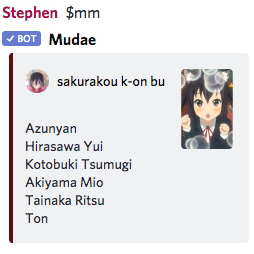
\includegraphics[scale=1]{images/collection.png}
  \caption{My collection.}
\end{figure}

\subsection{Mixed-Integer Linear Fractional Programming (MILFP)}
With cardinality essentially solved, we switch our focus to maximizing
kakera. We must first discuss theory to give context for our next program.

Recall we solved cardinality by writing the problem as a MILP. We now consider
\textit{fractional} programs, when our objective is a fraction with a linear
numerator and a linear denominator. We will warm-up by first considering
fractional constraints. Suppose we have a constraint of the form:
\[ \frac{a_1 x_1 + a_2 x_2 + \dots}{b_1 x_1 + b_2 x_2 + \dots} \leq c \]
If we assume that the denominator has the same sign (we can assume positive,
if the denominator is negative we can negate the denominator and negate the
numerator), then we can multiply both sides by the denominator without changing
the inequality.
\begin{align*}
  a_1 x_1 + a_2 x_2 + \dots &\leq c(b_1 x_1 + b_2 x_2 + \dots) \\
  (a_1 - c b_1) x_1 + (a_2 - c b_2) x_2 + \dots & \leq 0
\end{align*}
The same trick works for \( \geq \) or \( = \), of course. If the
constraint is equality, there does not need to be the requirement
that the denominator keeps the same sign because the sign won't
switch when multiplying across. If the denominator is 0, then the
multiplication will be 0, forcing the numerator to be 0.

\subsubsection{Charnes-Cooper}
We now consider how to turn a fractional objective into linear programming.
Suppose we want to maximize \( \frac{a_0 + a_1 x_1 + a_2 x_2 + \dots}{b_0 + b_1
x_1 + b_2 x_2 + \dots} \) subject to constraints of the form \( c_1 x_1 + c_2
x_2 + \dots \leq d \). We cannot do the same multiplication trick because there
is only one side of the objective. We instead create a new variable \( y_0 =
\frac{1}{b_0 + b_1 x_1 + b_2 x_2 + \dots} \) which represents the denominator.
As usual, the denominator must stay the same sign and be nonzero. Using this
new variable, we transform the objective:
\begin{align*} 
  \text{maximize }
  &\frac{a_0 + a_1 x_1 + a_2 x_2 + \dots}{b_0 + b_1 x_1 + b_2x_2 + \dots} \\
  &= (a_0 + a_1 x_1 + a_2 x_2 + \dots) y_0 \\
  &= a_0 y_0 + a_1 y_0 x_1 + a_2 y_0 x_2 + \dots
\end{align*}
The problem is that we have variables multiplied by each other, which
is not linear. However, we can be clever and substitute \( y_i = y_0
x_i \) in order to make the problem linear. Our objective has already
been transformed, and for each constraint, we multiply on both sides by
\( y_0 \) to force it into the terms of the newfound substitution.
\begin{align*}
  c_1 x_1 + c_2x_2 + \dots &\leq d  \\
  = c_1 y_0 x_1 + c_2 y_0 x_2 + \dots &\leq d y_0 
\end{align*}

Finally, we need to enforce the constraint that \(
y_0 \) is the denominator. We can convert fractional
constraints into linear constraints by multiplying across:
\begin{align*}
  y_0 &= \frac{1}{b_0 + b_1 x_1 + b_2 x_2 + \dots} \\
  b_0 y_0 + b_1 y_0 x_1 + b_2 x_2 y_0 + \dots &= 1
\end{align*}

With the objective, constraints, and denominator prepared,
we now make the substitution. The original program was:
\begin{align*}
  \text{maximize } 
  &\frac{a_0 + a_1 x_1 + a_2 x_2 + \dots}{b_0 + b_1 x_1 + b_2x_2 + \dots} \\
  \shortintertext{subject to:}
  &c_1 x_1 + c_2 x_2 + \dots \leq d 
  \shortintertext{With the substitution \( y_i = y_0 x_i \) this becomes}
  \text{maximize } 
  &a_0 y_0 + a_1 y_1 + a_2 y_2 + \dots \\
  \shortintertext{subject to:}
  &c_1 y_1 + c_2 y_2 + \dots \leq d y_0 \\
  &b_0 y_0 + b_1 y_1 + b_2 y_2 + \dots = 1
\end{align*}

We essentially get the same program! The only differences is that we change
the objective to just the numerator, and multiply each constant by \( y_0
\). Lastly, we turn the denominator into a new constraint. In terms of the
compact matrix-vector way to write a linear program, our original objective was
essentially \( \frac{\bm{c}_1^T \bm{x}}{\bm{c}_2^T \bm{x}} \) where the vector
\( \bm{x} \) is \( \begin{bmatrix} 1 & x_1 & x_2 & \dots & x_n \end{bmatrix}^T
\) to account for the constant term. Our constraints can be represented in a
matrix \( A \) such that \( A \bm{x} \leq \bm{b} \). After the transformation,
\( \bm{x} \) becomes \( \bm{y} = y_0 \bm{x} \) and the objective becomes just
the numerator, \( \bm{c}_1^T \bm{y} \). We add the vector \( -\bm{b} \) as
the leftmost column of the matrix and set \( \bm{b} = \vec{0} \). Finally, we
add the denominator \( \bm{c}_2^T \) as a row to the matrix, and \( 1 \) to
\( \bm{b} \) to turn the denominator into a constraint.

If we solve the new program, then we get solutions to \( \bm{y}
\). To get the final solution, we can compute \( \bm{x} \) by just
reversing the transformation, \( \bm{x} = \frac{1}{y_0} \bm{y} \).

This process is called \textit{Charnes-Cooper} and works great for continuous
variables, but we quickly run into a problem for mixed-integer problems.
Recall that we do the substitution \( y_i = y_0 x_i \). \( y_0 \) is a
continuous variable, and \( x_i \) is a discrete variable. What the heck is
\( y_i \) then? If we let \( y_i \) be a continuous variable, that doesn't
work because there's no guarantee that after we divide by \( y_0 \) we'll
get an integer---\( y_i \) is free to take on many different values, not
just multiples of \( y_0 \). Meanwhile if \( y_i \) is a discrete variable,
that doesn't work because \( y_0 \) can take on many different continuous
values. So \( y_i \) is ill-defined. In our particular case, however, \( x_i
\) is a binary variable meaning it's only ever 0 or 1. If there's only two
possibilities, can't we somehow force \( y_i \) to equal \( y_0 x_i \)?

\subsubsection{Glover's Linearization}
The general technique is called \textit{Glover's linearization},
\enquote{linearization} because it converts a nonlinear term into a linear
term. Suppose \( \bm{x} \) is a vector of binary variables and \( \bm{y}
\) is a vector of continuous variables. We wish to create a new continuous
variable \( z_i = g_i(\bm{x}, \bm{y}) \bm{x}_i \), where \( g_i(\bm{x},
\bm{y}) \) is a linear function of the variables. We assume that it does not
contain \( x_i \) since \( x_i^2 = x_i \) (\( 0^2 = 0 \), \( 1^2 = 1\)) and
that it does not contain constants (since multiplying by \( x_i \) would
be linear). We define \( L \) to be the minimum value of \( g_i \) on the
\textit{relaxation} of the domain \( X \), \( X^R \), where the relaxation
is the domain with the integer requirements removed, or \enquote{relaxed}.
We define \( U \) to be the maximum value of \( g_i \) on \( X^R \).
In order to enforce that \( z \) is the product of \( g_i \) and \( x_i \),
we enforce two constraints:
\begin{align}
  L_i x_i \leq z_i &\leq U_i x_i      \label{eq:cond1} \\ 
  g_i(\bm{x}, \bm{y}) - U_i (1 - x_i) \leq z_i &\leq 
  g_i(\bm{x}, \bm{y}) - L_i (1 - x_i) \label{eq:cond2} 
\end{align}

To see why this works, we can simply examine both cases. If \( x_i = 0
\) then the first constraint yields \( 0 \leq z_i \leq 0 \), forcing \(
z_i = 0 \). The second constraint is then \( g_i(\bm{x}, \bm{y}) - U_i
\leq z_i \leq g_i(\bm{x}, \bm{y}) - L_i \). \( g_i(\bm{x}, \bm{y}) -
U_i \) must be less than or equal to zero since \( U \) is the maximum
value, and similarly, \( g_i(\bm{x}, \bm{y}) - L_i \) must be greater
than or equal to zero since \( L \) is the minimum value. \( z_i = 0 \)
thus necessarily satisfies the second constraint.

If \( x_i = 1 \), then the second constraint yields \( g_i(\bm{x}, \bm{y}) \leq
z_i \leq g_i(\bm{x}, \bm{y}) \), forcing \( z_i = g_i(\bm{x}, \bm{y}) \). The
first constraint reduces to \( L_i \leq z_i \leq U_i \), which is satisfied by
the definition of \( L \) and \( U \). Thus, the two constraints force \( z_i =
g_i(\bm{x}, \bm{y}) x_i \) for any value of \( x_i \).

\subsubsection{Solving MILFPs}
We can now solve mixed-integer linear fractional programs. We first apply
Charnes-Cooper to obtain a non-linear integer program. We then apply Glover's
linearization to form a mixed-integer linear program. While this technique
is useful in the sense that we only need to solve one MILP, it significantly
increases the problem size. If the original problem had \( I \) continuous
variables, \( J \) binary variables, and \( K \) constraints, we add \(
\underbrace{J}_{\text{Glover's}} + \underbrace{1}_{\text{denominator}}
\) new continuous variables and \( \underbrace{3J}_{\text{Glover's}} +
\underbrace{1}_{\text{denominator}} \) new constraints. We add 3 constraints
instead of 4 because the denominator is necessarily positive, so \( L = 0 \)
and thus \( L_i x_i \leq z_i \) becomes \( 0 \leq z_i \), which is usually
implicit in linear programming.

\subsection{\texttt{\$antidisablelist} Optimization and Expected Value}
Before we can apply MILFPs to our problem of maximizing kakera, we must
formulate the program in the first place. Before we formulate the problem,
we introduce a new mechanic: \textit{antidisable} lists. We can antidisable
up to 500 series, where antidisabling a series means that it is no longer
disabled. This is irrelevant if we want to maximize the number of characters
disabled as we did in the previous section, but is now relevant for maximizing
kakera value---it is conceivable that we disable a bundle with many low-value
characters and then selectively antidisable the series that contain high-value
characters. We can implement this mechanic by introducing a new binary variable
\( z_i \) which represents whether the \( i \)th series is disabled or not.
We have that the sum of \( z_i \) is less than or equal to 500, and that \(
z_i \leq y_i \) since we can't antidisable the series if the series isn't
disabled. Finally, we replace \( y_i \) in the objective with \( y_i - z_i \)
to \enquote{zero-out} antidisabled series. What is our objective, anyways?
Instead of maximizing the number of characters disabled, we want to maximize
kakera. However, our model for kakera value is incredibly nonlinear. The best
we can do is use a heuristic, and the simplest is probably the expected value
of the kakera distribution. This corresponds to maximizing \( \E[X] \), which
is of course not maximizing \( \E[X_{30}] \), but a higher \( \E[X] \) should
mean higher character values overall. How do we formulate this objective of
maximizing expected value? Let \( t_i \) be the total kakera value of the \( i
\)th series. Then the expected value \( \E[X] = \frac{\sum t_i (1 - y_i)}{\sum
w_i (1 - y_i)} \) because \( y_i \) is whether a series is \textit{disabled},
so \( 1 - y_i \) is 1 if it is active, and 0 if the series is disabled. With
the objective complete, we make one last modification before formulating the
MILFP. Recall that the original linear program never explicitly enforced that
disabling a bundle disables the series it contains. That was fine for the old
objective of maximizing characters, but in this case it might be advantageous
to not disable---since it is essentially a free antidisable. We must therefore
enforce that \( y_i \geq x_j \) for each \( x_j \) that contains \( y_i \).
\begin{table}[h!]
  \centering
  \begin{tabular}{|c|c|}
    \hline
    name & variable \\
    \hline \hline
    \( x_i \) & \( i \)th bundle disabled or not \\
    \( y_i \) & \( i \)th series disabled or not \\
    \( z_i \) & \( i \)th series antidisabled or not \\  
    \( s_i \) & size of the \( i \)th bundle \\
    \( w_i \) & number of wa characters in the \( i \)th series \\
    \( t_i \) & total kakera value of the \( i \)th series \\ \hline
  \end{tabular}
  \caption{Variable names.}
\end{table}

\begin{align*}
  \tag{expected value program} \label{eq:expected_value}
  \text{maximize } &\frac{\sum t_i (1 - (y_i - z_i))}{\sum w_i (1 - (y_i - z_i))} 
  && \text{(expected value)} \\
  \shortintertext{subject to:}
  \sum& x_i \leq K && \text{(can only pick \( K = 10 \) bundles)} \\
  \sum& s_i x_i \leq 20000 && \text{(overlap limit)} \\
  \sum& z_i \leq 500 && \text{(antidisable limit)} \\
  \shortintertext{for each \( y_i \):}
  \sum_{j | y_i \in x_j}& x_j \geq y_i && 
  \text{(if \( y_i \) is disabled, at least one bundle disables it)} \\
                        & y_i \geq x_j && 
  \text{(disable \( y_i \) if at least one bundle disables it)} \\
                        & z_i \leq y_i &&
  \text{(can't antidisable if series isn't disabled)} \\
  &x_i, y_j, z_k \in \{0, 1\} && \text{(\( x \), \( y \), and \( z \) are binary variables)}
\end{align*}

Before we blindly apply our MILFP solving technique we notice that \( x_i
\) does not appear in the objective. In the continuous case, we essentially
discard the old variables and replace all of them with the transformed
variables, but in the mixed case we keep the old binary variables to enforce
the constraints on the transformed variables. We therefore save constraints
and variables if we simply don't multiply inequalities on both sides by the
denominator, and because we skip the multiplication we don't need to transform
\( x_i \) at all. A bit of ambiguity is whether we apply constraints like \(
\sum z_i \leq 500 \) to the transformed \( z_i \) or the binary \( z_i \). \(
z_i \) (and \( y_i \)) are essentially unconstrained if the constraints are
written entirely in the form of their transformed versions, and take their
values through the constraints in Glover's linearization. It is therefore
more consistent with \( x_i \), simpler, and more efficient to enforce the
constraints on the binary versions rather than the transformed versions.

We denote the continuous denominator variable for Charnes-Cooper as \( d \)
and we denote the transformed variables \( y'_i = d y_i \) and \( z'_i = d z_i
\). We must also determine the upper and lower bounds of \( d \) for Glover's
linearization. The denominator is one over the sum of the characters of the
series that are not disabled, so it is nonnegative (there would have to be
infinite characters to make \( d = 0 \)) and its largest value is when the
number of characters is the smallest, when as many characters as possible are
disabled. There is a hard limit of \( 90\% \) of characters disabled, so \(
d \) is bounded, and a simple upper bound is 1. The transformed program will
look very similar to the base program:
\phantomsection % not sure why I need this, but I do
\begin{align*}
  \tag{linearized} \label{eq:milfp}
  \text{maximize } &\sum t_i (d - (y'_i - z'_i))
  && \text{(numerator of expected value)} \\ 
  \shortintertext{subject to:}
  \sum& w_i (d - (y'_i - z'_i)) = 1 && \text{(denominator of expected value)} \\
  \sum& x_i \leq K && \text{(can only pick \( K = 10 \) bundles)} \\
  \sum& s_i x_i \leq 20000 && \text{(overlap limit)} \\
  \sum& z_i \leq 500 && \text{(antidisable limit)} \\
  \shortintertext{for each \( y_i \):}
  \sum_{j | y_i \in x_j}& x_j \geq y_i && 
  \text{(if \( y_i \) is disabled, at least 1 bundle disables it)} \\
                        & y_i \geq x_j && 
  \text{(disable \( y_i \) if at least 1 bundle disables it)} \\
                        & z_i \leq y_i &&
  \text{(can't antidisable if series isn't disabled)} \\
  \shortintertext{for each \( y_i \) and \( z_i \), call the variable \( v_i \):} 
  L v_i \leq v'_i & \leq U v_i
                  && \text{(\hyperref[eq:cond1]{1st condition of Glover's})} \\
  d - U(1 - v_i) \leq v'_i & \leq d - L(1 - v_i)  
                  && \text{(\hyperref[eq:cond2]{2nd condition of Glover's})} \\
  &x_i, y_j, z_k \in \{0, 1\} && \text{(\( x \), \( y \), and \( z \) are binary variables)} \\
  &d, y'_i, z'_j \in  [L, U] && \text{(continuous variables)} \\
\end{align*}

The program is pretty sensitive to \( L \) and \( U \). It is simplest to pick
\( L = 0 \) since that removes a constraint (linear programs implicitly have
nonnegative constraints). How does one determine \( U \)? We can simply use
the definition, the largest value on the relaxation. If we relax the problem
we get a linear program, whose objective is to \textit{minimize} \( \sum w_i
(1 - (y_i - z_i)) \) since \( d \) is one over that expression. Since linear
programming is polynomial time, it will run much quicker than the MILFP. Even
with the tight upper bound of \( U = 0.0002 \), the MILP does not converge in
any reasonable amount of time. One must therefore restrict the running time
and forgo convergence. It is also helpful to reduce the number of variables,
for example, to restrict the bundles being disabled to the top 100 largest
bundles as the smaller bundles necessarily have less of an effect.

Another trick is to re-write the constraint that \( y_i \geq x_j \). It looks
innocent because of the notational trick: I mean that \( y_i \) needs to be
greater than \textit{each} \( x_j \) such that \( y_i \in x_j \). In the
worst case each series could add up to the number of bundles to the number of
constraints. The intuition is that we want to force \( y_i \) to be 1 if any \(
x_j \) is 1, or if \( x_1 + x_2 + \dots + x_n \) is greater than 0 (addition
is essentially bitwise OR). We can't just enforce that \( y_i \geq x_1 + x_2 +
\dots + x_n \) because if multiple \( x_j \) are on, \( y_i \) can only be at
most 1. So we can divide by the same thing to \enquote{normalize} the addition
into a boolean. We then enforce \( y_i \geq \frac{x_1 + x_2 + \dots + x_n}{x_1
+ x_2 + \dots + x_n} \) which is not equivalent to enforcing that \( y_i \geq
1 \) because of the case where all \( x_j \) are 0. To see the difference,
multiply across to linearize the constraint: \( (x_1 + x_2 + \dots + x_n) y_i =
x_1 + x_2 + \dots + x_n \). If each \( x_j \) is 0, then the constraint reduces
to \( 0 = 0 \), which is trivially satisfied. The other constraint that \( \sum
x_j \geq y_i \) then forces \( y_i \) to be 0, which must be true if none of
the bundles which contain it are disabled. If at least one of the \( x_j \)'s
is 1, then \( y_i \) is forced to be 1 to make \( y_i \geq \frac{x_1 + x_2 +
\dots + x_n}{x_1 + x_2 + \dots + x_n} \) true. Meanwhile the second constraint
is now redundant as it reduces to \( \sum x_j \geq 1 \), which is satisfied as
we know at least one of the \( x_j \) is 1. Although the new constraint works
to enforce the behavior we want, the product between \( y_i \) and the sum of
\( x_j \)'s then needs to be linearized with Glover's, which we can do all at
once instead of for each \( x_j \):
\begin{align}
  g_i(\bm{x}, \bm{y}) &= x_1 + x_2 + \dots + x_n \\  
  L_i y_i \leq y'_i &\leq U_i y_i                     \label{eq:glover1} \\
  g_i(\bm{x}, \bm{y}) - U_i (1 - y_i) \leq y'_i &\leq 
  g_i(\bm{x}, \bm{y}) - L_i (1 - y_i)                 \label{eq:glover2} \\ 
  y'_i &\geq g_i(\bm{x}, \bm{y})                      \label{eq:disable}
\end{align}

\( L \) is clearly 0 if all \( x_j \) are 0 and a simple upper bound for \( U
\) is simply the number of \( x_j \) which contain \( y_i \), \( n \). Using
these new bounds, we can simplify the 5 inequalities considerably. The left
half of \eqref{eq:glover1}, \( L_i y_i \leq y'_i \), becomes \( 0 \leq y'_i
\), which is again implicit in the definition of \( y'_i \), so it can be
removed. For the left half of \eqref{eq:glover2}, we consider the two cases
of \( y_i \). If \( y_i = 0 \) then \( y'_i = 0 \) from the right half of
\eqref{eq:glover1} and \( g_i(\bm{x}, \bm{y}) - U_i \leq 0 \) follows from
the definition of \( U \). If \( y_i = 1 \), then the inequality reduces to
\( g_i(\bm{x}, \bm{y}) \leq y'_i \) which is exactly \eqref{eq:disable}.
Thus, because it is redundant in either case, we can remove this constraint
as well. Finally, we notice that if \( L = 0 \), then the right side of
\eqref{eq:glover2} reduces to \( g_i(\bm{x}, \bm{y}) \leq y'_i \), which can
be combined with \eqref{eq:disable} to yield \( y'_i = g_i(\bm{x}, \bm{y}) \).
Since this is an equality constraint with just one variable, we can avoid
creating a new continuous variable for \( y'_i \) by just substituting its
value wherever \( y'_i \) occurs, in this case just \( y'_i \leq U_i y_i \).

Recall that we started by adding possibly \( n \) new constraints per series,
where \( n \) is the number of bundles which contain the series. Using the
re-write and Glover's linearization, we turned \( O(n) \) into \( O(1) \) by
adding at most 5 constraints and 1 continuous variable. Finally, with the
observations pruning extraneous constraints, we add just 1 constraint:
\[ g_i(\bm{x}, \bm{y}) \leq U_i y_i \]

After running for 2 hours on
\href{https://documentation.tjhsst.edu/machines/other/snowy}{Snowy}, the
linear program found an expected value of 75.679 compared to the original
61.702 and a model expected value of 429.839 compared to 322.371. A 14
kakera improvement in the kakera distribution is nothing extraordinary,
but that difference is heavily magnified by the model, increasing
the average value per claim by more than 100 kakera.

\subsubsection{Linear Regression}

While expected value is a decent heuristic, can we do better? Our objective must
be linear, because we are using linear programming. Is there a way to turn a nonlinear
function into a linear function? Well, the best we can do is to fit a line. We fit
this line with \textit{linear regression}---my derivation can be found 
\href{https://activities.tjhsst.edu/computervision/lectures/Tensor_Calculus.pdf}{here}. 

Our objective is a mapping from the active series to the expected value of
the model. We can represent the active series as a bitstring of whether a
series is active or not, so the dimensionality of the input is the number
of series. We randomly and uniformly\footnote{What does it mean to generate
something \enquote{uniformly}? Each thing in the space must have an equal
probability of being picked. There are \( 2^n \) bitstrings of length \(
n \), and if we generate bit by bit, with each bit having a 0.5 chance to
be 1, then each string has a \( \frac{1}{2} \cdot \frac{1}{2} \cdot \ldots
\cdot \frac{1}{2} = \frac{1}{2^n} \) chance of being generated.} generate a
bit string by generating each bit at a time, where each bit has a 0.5 chance
to be 1 and a 0.5 chance to be off. We then extract a random variable from
the resulting character data and feed the random variable to our model,
which computes the expected value. Doing this multiple times to generate a
dataset, we fit linear regression to the data which gives us a linear function
representing the relationship between the series variable and the expected
value. We can then use this line as the objective of our linear program.

The benefits over the MILFP for expected value is that our linear regression
might be more aligned with the model expected value and that we do not increase
the problem size. Despite the significantly reduced problem size, it still
does not converge in time. In terms of the results, I generated a dataset with
10,000 rows. The linear regression has a \( R^2 \) of 0.953 on the training
dataset but only a 0.586 \( R^2 \) on the testing dataset of size 1,000,
suggesting a lack of generalization.\footnote{I am aware that a higher score
on the training dataset relative to the testing dataset is a classic sign of
\textit{overfitting}. However, in this situation the linear regression is by
definition underfitting---the relationship is highly nonlinear, so a linear
model is not the right choice.} As a result of this lack of alignment, the
expected value of the kakera distribution is actually lower and the model
expected value is approximately the same.

\subsection{Conclusion}
I began this section optimistically, stating that NP-hard is not a death
sentence---problems can still be tractable in the average case. My optimism is
tempered by the lack of convergence I have witnessed for the latter programs.
To summarize, we will compare the sizes of each of the programs developed. If
\( B \) is the number of bundles and \( S \) is the number of series, then:
\begin{table}[h!]
  \centering
  \begin{tabular}{|c|c|c|c|}
    \hline
    name & binary variables & continuous variables & constraints \\
    \hline \hline
    \multirow{2}{5em}{\hyperref[eq:char]{cardinality}}
    & \( (B + S) + S \) & 0 & \( 1 + 1 + S \) \\
    & \( B + 2S \) & 0 & \( S + 2 \) \\
    \hline
    \multirow{2}{5em}{\hyperref[eq:expected_value]{fractional program}}
    & \( [B + 2S] + S \) & \( 0 \) & \( [S + 2] + 1 + S + S \) \\
    & \( B + 3S \) & \( 0 \) & \( 3S + 3 \) \\
    \hline
    \multirow{2}{5em}{\hyperref[eq:milfp]{linearized program}}
    & \( B + 3S \) & \( 2S + 1 \) & \( [3S + 3] + 3(2S) + 1 \) \\
    & \( B + 3S \) & \( 2S + 1 \) & \( 9S + 4 \) \\
    \hline
  \end{tabular}
  \caption{Program sizes.}
\end{table}

The sizes grow quite quickly from the cardinality program to the final MILFP.
Likewise, the cardinality program converges in less than 10 seconds while I
have no idea how long the expected value MILFP takes to converge---all I can
say is that it's longer than 24 hours. Would the
\href{https://optimization.mccormick.northwestern.edu/index.php/Mixed-integer_linear_fractional_programming_(MILFP)}
{parametric algorithm} instead of the reformulation-linearization
explored in this section be more efficient? I encourage the reader to
see for themselves. Whatever the case, the problem is rich for future
exploration---the optimization of an incomplete \textit{heuristic} hasn't
even been solved! Can the connection between optimizing disablelists
while taking into account the probabilistic model ever be completed in
full? I wouldn't have written \pageref{here2} pages if I thought that
the task was truly impossible. \( \qed \)

\newpage

\section{Extensions and Future Work}
Despite the length of this paper, there
remains many avenues for future research.
\begin{enumerate}
  \item \textit{A proper way to maximize expected value.}
    In order to optimize disablelists, we use expected value of the
    kakera distribution as a heuristic for the expected value of the
    model. Can we get better performance with quadratic programming
    or convex optimization techniques? Deep learning?

  \item \textit{A provably optimal model over a known timescale.}
    As stated before, if the timescale is known then the optimal
    model changes (because expected value is optimal over an infinite
    timescale). Can we create a model that is optimal for short timescales?

  \item \textit{Empirically inferring taste distributions.}
    People do not act to maximize expected kakera value. They have characters
    they like, which they might claim without regard to its quantitative value.
    Suppose we assume that these people are not simply irrational but have a
    different value distribution, a phenomenon often called \textit{taste}. Can
    we infer a person's taste distribution from their actual claiming behavior?

  \item \textit{Implementing more Mudae mechanics.}
    Wishlists, badges, kakera reacts, etc.

  \item \textit{A Discord bot.}
    While self-botting is against the terms of service, a discord bot which
    one could invoke for advice would be nicer than interacting with the CLI.

  \item \textit{A class for random variables.}
    It would be cleaner to create a \texttt{RandomVariable} class which
    contained all the helper methods like PMF, CMF, expectation, etc. One
    could then instantiate this class by providing a list of values and
    their probabilities. That would be nicer than carrying around lists
    everywhere and managing functions.
\end{enumerate}

\section{Sources}
\begin{enumerate}
  \item \href{https://en.wikipedia.org/wiki/Inverse_transform_sampling}
    {The inverse transform for sampling---Wikipedia}
  \item \href{https://activities.tjhsst.edu/sct/lectures/2021/2020_10_23_FFT_handout.pdf}
    {My convolution and the FFT lecture}
  \item \href{https://plato.stanford.edu/entries/paradox-stpetersburg/}
    {St. Petersburg Paradox---Stanford Encyclopedia of Philosophy}
  \item \href{https://people.seas.harvard.edu/~yaron/AM221-S16/lecture_notes/AM221_lecture18.pdf}
    {Maximum set cover}
  \item \href{https://www.python-mip.com/}
    {Python mixed-integer linear programming library}
  \item \href{http://web.mit.edu/15.053/www/AMP-Chapter-04.pdf}
    {Duality in linear programming}
  \item \href{http://lpsolve.sourceforge.net/5.1/ratio.htm}
    {Ratios in linear programming}
  \item \href{https://optimization.mccormick.northwestern.edu/index.php/Mixed-integer_linear_fractional_programming_(MILFP)}
    {Solving mixed-integer linear fractional programs}
  \item \href{https://doi.org/10.1016/j.disopt.2004.03.006}
    {Glover's linearization}
  \item \href{https://glossary.informs.org/ver2/mpgwiki/index.php?title=Relaxation} 
    {Relaxation}
\end{enumerate}

\newpage

\section{Appendix}
\subsection{Secretary Problem} \label{subsec:secretary}
Mudae is very related to the
\href{https://www.smbc-comics.com/comic/percent}{secretary problem}. Suppose
you are a secretary interviewing job applicants. You have \( n \) candidates
and there is a clear ranking among the candidates, e.g. after interviewing
a candidate you can tell how they rank amongst the candidates you've
already interviewed. The twist is that you must choose to accept or reject
a candidate immediately after their interview. What should be your strategy
to maximize the probability of picking the best candidate?

It can be shown that the optimal strategy is of the form \enquote{always
reject the first \( r \) candidates, then pick the first candidate who is
better than all the candidates you've rejected.} Interestingly enough, \( r
\) approaches \( \frac{n}{e} \) as \( n \) approaches \( \infty \), so you
should reject the first \( \frac{1}{e} \) fraction of candidates or about
the first \( 36.8\% \). The probability of picking the best candidate is
also \( \frac{1}{e} \), regardless of the size of \( n \).

How is this problem related to Mudae? Both are based off the immediate decision
making for a given candidate. Consider the following two solutions for the
secretary problem: one picks the best candidate with a 50\% chance, but picks
the absolute worst candidate the rest of the time. The other picks the best
candidate with a 49\% chance, and picks the second best the rest of the time.
Is the first strategy really better than the second strategy? If one weights
the candidates by some quantitative value with a known distribution and wants
to maximize the \textit{expected value} rather than simply the maximum value,
then the problem reduces to Mudae.

\newpage

\subsection{Conditional Probability} \label{subsec:conditional}
\begin{definition}
  The probability that an event \( A \) happens \textit{conditional} on \( B \)
  is denoted \( p(A|B) \), i.e. the probability \( A \) happens \enquote{given}
  \( B \) happens. This should not be confused for \( p(A \cap B) \),
  the probability \( A \) happens \textit{and} \( B \) happens.
\end{definition}

\begin{corollary}
  \[ p(A|B) = \frac{p(A \cap B)}{p(B)} \]
\end{corollary}
\begin{proof}
  We will use an informal (and therefore loose) definition of probability as
  the number of ways for something to occur over the total number of ways.
  Since we know \( B \) occurs, the total number of ways is \( p(B) \).
  The number of ways \( A \) occurs is the number of events where \( A \)
  occurs \textit{and} \( B \) occurs, because we know \( B \) occurs.
\end{proof}

One way to picture this is to imagine a Venn diagram in a rectangle, where
the rectangle is the universe of all possible events, one circle is \( A
\), and the other \( B \). If we restrict our universe to \( B \) since we
know \( B \) occurs, then the ways \( A \) occurs is the intersection of
\( A \) and \( B \), \( A \cap B \). The ways \( B \) occurs is just \( B
\)'s circle, \( p(B) \).

\begin{theorem}
  Bayes' Theorem, i.e. switching conditional probabilities: 
  \[ p(A|B) = \frac{p(B|A) p(A)}{p(B)} \]
\end{theorem}
\begin{proof}
  From the definition of conditional probability we know
  \begin{align*}
    p(A|B) &= \frac{p(A \cap B)}{p(B)}
    \shortintertext{Multiplying by \( p(B) \) on both sides,}
    p(A|B)p(B) &= p(A \cap B)
    \shortintertext{Since we know \( A \cap B = B \cap A \),}
    p(B \cap A) &= p(A|B)p(B) = p(B|A)p(A)
    \shortintertext{where the latter identity comes from the original identity.
    Thus,}
    p(A|B) &= \frac{p(B|A)p(A)}{p(B)} && \qedhere
  \end{align*}
\end{proof}

One way to interpret this theorem is suppose \( A \) is our hypothesis and
\( B \) is a new piece of data. Then \( p(A|B) \) is how confident we are in
the hypothesis given the new piece of data, \( p(B|A) \) is how probable the
data is under our hypothesis, \( p(A) \) is the \textit{prior} probability in
our hypothesis (how sure we are in the hypothesis before piece of data), and
\( p(B) \) is how probable the data is overall (which, in practice, is often
intractable: how do we compute the probability over \textit{all} hypotheses?).

\subsection{\enquote{General} Rolls Model} \label{subsec:general}
We have two key assumptions:
\begin{enumerate}
  \item Use at most one \texttt{\$rolls} per claim cycle.
  \item \( k^* \) is less than \( \E[X_B] \) 
\end{enumerate}
The second assumption can be checked empirically and is only
for making introspection easier. Can we formulate an optimal
model with an unlimited usage of \texttt{\$rolls} per claim?

The observation is that we want to avoid low kakera values, regardless of
when they occur. For example, the minimum possible value is 32. Suppose we
are about to claim a 32 value character, and use \texttt{\$rolls} to avoid
this fate. However, we get unlucky and all 10 of our new rolls were 32 yet
again. Should we use \texttt{\$rolls} again, or at some other time? Well, in
what other situation would it be as beneficial to avoid the minimum possible
value? Ignoring the fact that we've already used \texttt{\$rolls}, clearly
we should use it again.

The probability of being about to claim \( k = 32 \) is the probability we're
at the last layer times the probability of rolling \( k \), \( p(\text{emit
at } 1) p_Z(k) \). Then the chance we use \texttt{\$rolls} once is \( p(1)
p_Z (k) ( 1 - p_Z(k) ) \) since we if we use it exactly once, we first
roll \( k \) then roll anything higher than \( k \), which is anything
except \( k \). The chance we use it twice is \( p(1) p_Z(k)^2 (1 - p_Z(k))
\), three times \( p(1) p_Z(k)^3 (1 - p_Z(k)) \), and so on. This is a
geometric random variable with probability of success \( 1 - p_Z(k) \) (in
this case \enquote{success} is \textit{not} rolling \( k \) since that's
when we break out of using \texttt{\$rolls}). The expected value is then \(
\frac{p(\text{emit at} 1) p_Z(k)}{1 - p_Z(k)} \), which is how many times we
expect to use \texttt{\$rolls} if we use it only on the minimum value. If
this is less than \( \frac{1}{8} \), then we can also use \texttt{\$rolls}
on the second smallest value. In general, we find the largest \( k^* \) such
that \( \frac{p(\text{emit at} 1) F_Z(k^*)}{1 - F_Z(k^*)} \) is smaller than
\( \frac{1}{8} \) (since the chance we \enquote{enter} a cycle of using
\texttt{\$rolls} is \( p(1) F_Z(k^*) \) and the chance we break out is if
we roll something higher than \( k^* \), a \( 1 - F_Z(k^*) \) chance). We
find this \( k^* \) with binary search like the standard rolls model, and if
we binary search on indexes the time is \( O(\log n) \) rather than binary
searching on values, \( O(\log^2 n) \) because of the \( O(\log n) \) cost
to compute the CMF at a value not in the range.

This has the effect of lowering \( k^* \) relative to the standard rolls model,
68 versus 72. This is because more probability mass is concentrated in the
lower kakera values, since we can use \texttt{\$rolls} a theoretically infinite
times on each kakera value smaller than \( k^* \). It also slightly raises the
expected value since we use \texttt{\$rolls} on the worst situations, 322.371
for the general model versus 322.036 for the standard model.

Unfortunately, the actual game limits \texttt{\$rolls}
to once per interval, so this model is simply an
interesting demonstration of geometric random variables.

\label{here2}

% \printbibliography
\end{document}
